\section{Cover decidability}

\subsection{Set-up}

\ifintuition
\subsection{Intuition}

Our aim is to prove the decidability of the coverability problem for BNRA which can only send a single value in each broadcast. The constructions will actually lead us to a decidability proof for specifications of two different types, both subsuming the coverability specification.

\paragraph*{Step 1 : simplification} In Lemma~\ref{lem:simple-reduction} we prove that all protocols, even those which can apply several operations when receiving a broadcast, can be simulated by a protocol with a single operation upon reception of a message and no $*$ operation. A previous lemma already allowed us to remove $\diseqtestact$, thus we only have to prove decidability for systems with one operation per reception and only $\enregact$ and $\eqtestact$ operations.

Lemma~\ref{lem:simple-reduction} is placed within the decidability proof as the constructions defined there may simplify the proof of the lemma (they allow us to prove that BRNA can simulate each other simply by proving that their local runs have the same behaviour).

\paragraph*{Step 2 : run decomposition} Say we have a global run $\rho$ in which an agent broadcasts a message $m_f$. We isolate the local run $u$ of the first agent $a$ broadcasting $m_f$.
In order to execute $u$, we need to receive a sequence of broadcast that matches the sequence of receive transitions in $u$. Let $v$ be a value appearing in $u$.

\begin{itemize}
	\item 
	Say $v$ is not an initial value of $u$, let $w \in \messages^*$ be the sequence of broadcasts received by $a$ with value $v$ in $u$. Then the exact value $v$ does not matter, all $a$ needs is to receive a series of broadcasts with the messages of $w$ all with the same value. This is possible if and only if there exists a global run $\run'$ and a value $v'$ such that $w$ is a subword of the series of broadcasts made in that run with value $v'$. Indeed, if there exists such a run, then $u$ can receive selected broadcasts from $\rho'$ (happening in parallel) in order to get the sequence $w$ of messages with the same value. Conversely, if $u$ receives a sequence $w$ all with the same value in $\rho$, then the prefix of $\rho$ ending just before the broadcast of $m_f$ by $u$ is a fitting candidate for $\rho'$.
	We do not take $\rho$ directly as witness as we want the runs to get shorter as we make the recursive calls.
	
	Here we have our first type of specification, given as a word $w \in \messages^*$. We ask that there exists a global run and a value $v'$ such that $w$ is a subword of the sequence of broadcasts made in the global run with value $v'$.
	
	
	\item 	
	Now suppose $v$ is an initial value of $u$. This situation is very different as other processes need $a$ to send some messages with this value in order to be able to send it back to him.
	The key observation is that once an agent $a'$ other than $a$ has managed to broadcast some message $m$ with value $v$, we have an unlimited supply of such broadcasts:
	Let $w$ be the series of messages broadcast by $a$ with value $v$ before $a'$ makes that broadcast, we now know that there is a global run which, if presented with an external series of broadcasts $w$ with the same value, can then broadcast $m$ with that value.
	We then extend this reasoning and consider the series of broadcast made with value $v$ through $\run$. It can be decomposed as  $(w_0, m_1, w_1, \ldots, m_\ell, w_\ell)$ where $w_0 \cdots w_\ell$ is the sequence of broadcasts made by $a$ with that value and the $m_j$ are placed at the moments where another agent manages for the first time to broadcast that message (from then on we have unlimited supplies of broadcasts with that value and message $m_j$). In particular $\ell \leq \size{\messages}$.
	
	All we have to do is to check for all $j$ that there exists a global run in which some agent broadcasts $m_j$ with a value $v$ that is not one of its initial ones, while having received a series of external broadcasts $w'$ which is of the form $w'_0\cdots w'_{j-1}$ where each $w'_i$ is obtained by adding some letters from $\set{m_0, \ldots, m_i}$ in $w_i$.
	If we have such a run, then with the copycat property we can add an  agent that copies 
	
	This forms our second type of specification, given by a decomposition $(w_0, m_1, w_1, \ldots, m_{j-1}, w_{j-1}, m_j)$, which asks for a run that broadcasts $m_j$ with some value $v'$ which it does not have initially, while receiving a series of  external broadcasts with value $v'$ that match $(w_0, m_1, w_1, \ldots, m_{j-1}, w_{j-1})$.
\end{itemize}   

We can decompose any run satisfying one of those specifications into a local run (the one of the agent having the value initially in the first case, the one of the first agent which manages to broadcast $m_j$ while not having the value initially in the second case) and some number of specifications satisfied by smaller runs.

Hence we can turn a global run satisfying a given specification into a finite tree where nodes are labelled by local runs and specifications of one of the two types above.

\subsection{Bounds on the size of the minimal decomposition}

The previous section provides witnesses for the satisfiability of specifications, in the form of a tree decomposition.

However it is not clear that there is any bound on the size of those trees.

To provide such bounds, we need several observations.
We say that a local run is cheaper than another one if the set of children it spawns in the decomposition tree is easier to achieve: every child of the first run is a subword of a child of the second one.

 First of all we use Lemma~\ref{lem:short-local-runs}, essentially stating that we can reduce any section of a local run of length more than $f(|\prot|)$, where $f$ is a primitive recursive function, to obtain a shorter and cheaper local run.
 This new run may broadcast less messages, thus we cannot say that every local run can be reduced to one of size $f(\size{\prot})$.
 However, we can say that if there exists a local run making some sequence of $N$ broadcasts, then there is one of size at most $Nf(\size{\prot})$, as we can reduce the sections of runs between those broadcasts.
 
 We now define a notion of altitude of a node, which is not the same as its depth in the tree. Intuitively we put the children of a node $n$ below it if $n$ has to receive messages from them (first case in the previous subsection) and above it if $n$ has to send messages to them (second case).
 The altitude of the root is $0$, and the altitude of a child of a node $n$  is  the one of $n$ minus one if it is of the first type of specification, plus one otherwise.
 
 Nodes of minimal altitude (except maybe the root) are nodes of the second type which only have children of the first type, hence all they have to do is broadcast one single message (given by their father). Hence their length is at most $f(\size{\prot})$. 
 
 Now assume we have a bound $M$ on runs of altitude $h$. A run of altitude $h-1$ sees at most $r$ different initial values. Hence it has at most $\size{\messages}r$ children of the second type, and for each corresponding specification it has to make at most $M$ broadcasts, as each of those children makes at most $M$ receiving actions.
 Moreover, if it is of the first type, it also has to provide broadcasts for its father, but again his father has altitude $h$, thus will require at most $M$ broadcasts.
 
 Overall a local run at altitude $h-1$ needs to make a series of at most $M(\size{\messages} r +1)$ broadcasts. If that can be done, it can be done by a local run of length at most $[M(\size{\messages} r +1)](f(\size{\prot})+1)$.
 
 As a result, we can bound the size of a node of altitude $h$ by $g(\size{\prot}, hmax-h)$, where $hmax$ is the maximal altitude of the tree and $g$ is a primitive recursive function.
 
 This allows us to bound $hmax$: indeed consider the branch reaching the highest point in the tree. Along that branch we can extract a sequence of nodes of the second type $\node_0, \ldots, \node_{hmax}$ such that $\node_i$ has altitude $i$ for all $i$. If there are some $i<j$ such that $\node_i$ and $\node_j$ produce the same broadcast but $\node_j$ is cheaper then we can reduce the branch.
 The bounds on the lengths of the $\node_i$ and the latter property allow us to bound $hmax$ with a function from the class $F_{\omega^k}$ with $k = \size{\Sigma} +1$ (see, for instance, \cite{SchmitzS2011upperHigman}).
 
 This also gives us a bound on the size of the root (which is also in $F_{\omega^k}$). From there we bound the minimal altitude of a node of this tree. The argument is that in order to reach a minimal altitude $hmin$ with a branch, we need to have along that branch a subsequence of nodes of the first type $\node_0, \ldots, \node_{-hmin}$ such that $\node_i$ has altitude $-i$. If there exist $i<j$ such that $\node_i$ broadcasts a subword of $\node_j$ we can reduce the branch. Otherwise, the same results on bad sequences of words  for the subword order allow us to bound the minimal altitude of a node in that tree with a function of $F_{\omega^k}$.
 As both the minimal and maximal altitudes in the tree are bounded by such functions, the size of a node of that tree is also bounded by such a function (using the bound on nodes based on their altitude). This is also a bound on the branching of the tree, as the number of children of a node is bounded by the number of values seen in its local run, thus by the size of that run.
 
 The number of different nodes along a branch is also bounded, hence also the size of that branch (if the same node appears twice we can reduce the branch).
 This lets us bound the overall size of the tree with a function of $F_{\omega^k}$, yielding decidability and complexity of the problem.

\subsection{Formal proof}
\fi

\textbf{For now we assume that the BRNA do not contain $*$ operations and apply only one operation for each message received. The general case reduces to this one (lemma \ref{lem:simple-reduction}).}

% \begin{definition}
% 	An ""external broadcast"" is a transition between two configurations $\config \extbr{m, v} \config'$ such that $m \in \messages$, $v \in \nats$ and for all $a \in \agents$, either $\config'(a) = \config(a)$ or there exists a transition $(\st{\config}(a),\rec{m}{j}{\anact},\st{\config'}(a))$
% 	such that $\data{\config'}(a, j') = \data{\config}(a, j')$ for all $j' \neq j$ and one of the following cases holds:
% 		\begin{itemize}
% 			\item $\anact = \quotemarks{\dummyact}$ 
% 			and $\data{\config'}(a,j) = \data{\config}(a,j)$
% 			\item $\anact = \quotemarks{\enregact}$ and $\data{\config'}(a,j) = v$
% 			\item $\anact = \quotemarks{\eqtestact}$ and $\data{\config'}(a,j) = \data{\config}(a,j) =v$
% 			\item $\anact = \quotemarks{\diseqtestact}$ and $\data{\config'}(a,j) = \data{\config}(a,j) \ne v$.
% 		\end{itemize}

%\subsubsection{Definitions}
\begin{definition}[Local runs]			
	A ""local configuration"" is a pair $(q, \localdata) \in Q \times ([1,r] \to \nats)$. Intuitively, it describes the configuration of a single agent. 

	An ""external broadcast"" from $(q,\localdata)$ to $(q',\localdata')$ with transtion $\atrans \in \transitions$ and value $\aval \in \nats$, denoted $(q,\localdata) \extbr{\atrans}{\aval} (q',\localdata')$, is defined when $\atrans = (q,\rec{m}{j}{\anact},q') \in \transitions$
	such that $\localdata(j') = \localdata(j')$ for all $j' \neq j$ and one of the following cases holds:
		\begin{itemize}
			\item $\anact = \quotemarks{\dummyact}$ 
			and $\localdata(j) = \localdata'(j)$
			\item $\anact = \quotemarks{\enregact}$ and $\localdata'(j) = v$
			\item $\anact = \quotemarks{\eqtestact}$ and $\localdata(j) = \localdata'(j)= v$
			\item $\anact = \quotemarks{\diseqtestact}$ and $\localdata(j) = \localdata'(j) \ne v$.
		\end{itemize}
	Said otherwise, $(q,\localdata) \extbr{\atrans}{\aval} (q',\localdata')$ when an agent in $(q,\localdata)$ may perform $\atrans$ when receiving a message of the right type with value $\aval$.

	An ""internal step"" from $(q,\localdata)$ to $(q',\localdata')$ with transition $\atrans \in \transitions$, denoted $(q,\localdata) \intstep{\atrans} (q',\localdata')$, is defined when $\atrans$ is either a "broadcast" or a "local test" and an agent in $(q,\localdata)$ may perform this transition in isolation and get to $(q',\localdata')$. 

	A ""local step"" $(q,\localdata) \step{} (q',\localdata')$ is either an "external broadcast" or an "internal step". 
	A ""local run"" is a sequence $\localrun$ of "local steps" $(q_0, \nu_0) \step{\locallabel_1} (q_1, \nu_1) \step{\locallabel_2} \cdots \step{\locallabel_k} (q_k, \nu_k)$, where for all $i$, $\locallabel_i \in \set{\extlabel{\atrans}{\aval} \mid \atrans \in \transitions, \aval \in \nats} \cup \set{\intlabel{\atrans} \mid \atrans \in \transitions}$. The sequence $\locallabel_1, \dots, \locallabel_k$ is called ""schedule"" of $\localrun$.

	The ""trace"" of a "local run" is the sequence $\trace{\localrun} \in (\messages \times \nats \times \set{in, out})^*$ containing the message types and values that it receives and broadcasts, $in$ indicating an "external broadcast" and $out$ a broadcast made in $u$.

	The ""input"" of a "local run" $\localrun$ is the sequence $\Input{\localrun} \in (\messages \times \nats)^*$ containing messages types and values of its "external broadcasts".
	Similarly, its ""output"", which we denote by $\Output{\localrun} \in (\messages \times \nats)^*$, is the sequence of messages of (internal) broadcasts steps made in $\localrun$.
	
	Given a value $v \in \nats $, the $v$-input $\vinput{\aval}{\localrun} $(resp. the $v$-output $\voutput{\localrun}{\aval}$) of $\localrun$ is defined as the sequence of messages of $\Input{\localrun}$ (resp. $\Output{\localrun}$) that have value $\aval$. Formally, $\vinput{\aval}{\localrun}$ is the word $m_0 \cdots m_{\ell} \in \messages^*$ such that $(m_0, \aval) \cdots (m_{\ell}, \aval)$ is the projection of $\Input{\localrun}$ on $\messages \times \set{\aval}$. 
\end{definition}


We start by proving that we may in fact get rid of local equality tests:

\begin{restatable}{lemma}{SimpleReduction}
	\label{lem:simple-reduction}
	There exists an exponential-time reduction from the "coverability problem" to the coverability problem on protocols with no "local equality tests" $\loc{i}{j}{=}$.
\end{restatable}

The proof can be found in Appendix~\ref{sec:proof-simple} \corto{A corriger}. In fact, the exponential cost of the reduction will have no impact the complexity results proven below.
In the following, we will assume that the considered protocol has no "local equality tests". 



\subsection{Decomposition trees}

A key ingredient of our construction is the decomposition of words of messages. Say we have an execution and a value $v$ such that the sequence of messages broadcast in that execution with value $v$ is $w$. Let $w'$ the subword of $w$ of messages sent by the agent $a$ which had that value originally. Let $m$ be the first message sent by another agent with value $v$. This means that from the messages sent by $a$ before there is a set of agents that receives some of these messages and eventually sends back message $m$ with value $v$. An important remark is that we can copy this set of agents many times to obtain as many broadcasts with message $m$ and value $v$ as we want from this point in the run.

In general, if an agent other than $a$ sends a message with value $v$ then we can add agents to obtain that message with that value as many times as we want.
Therefore, we will describe the sequences of messages sent with a value $v$ as tuples $(w_0, m_1, \ldots, m_\ell, w_\ell)$, where $w_0 \cdots w_\ell$ is the sequence of messages sent by the agent $a$ which has that value initially and the $m_i$ mark, for every message of $\messages$ the first moment at which some agent other than $a$ broadcasts it with value $v$ (if that happens).


\begin{definition}
	A ""decomposition"" is a tuple $\decsymb = (w_0, m_1, \ldots, m_\ell, w_\ell)$ with $w_0, \ldots, w_\ell \in \messages^*$, and $m_1, \cdots, m_\ell \in \messages$, with $m_i \neq m_j$ for all $i\neq j$. In particular we have $\ell \leq \size{\messages}$. The set of decompositions over $\messages$ is denoted $\decset{\messages}$.
	
	We say that a word $w \in \messages^*$ ""decomposes as"" $\decsymb = (w_0, m_1, \ldots, m_\ell, w_\ell)$ if $w = w'_0 w'_1 \cdots w'_\ell$ where for all $j$, $w'_j$ can be obtained from $w_j$ by adding some letters from $\set{m_1, \ldots, m_{j-1}}$.
	
	The language $\langdec{\decsymb}$ of $\decsymb$ is the set of words that decompose as $\decsymb$. We write $\langdecdown{\decsymb}$ for the subword closure of $\langdec{\decsymb}$.
	
	We define a preorder on decompositions:
	$\decsymb \subdec \decsymb'$ if $\langdecdown{\decsymb} \subseteq \langdecdown{\decsymb'}$.
\end{definition}


\begin{definition}
	\label{def:tree-unfolding}
	A ""tree unfolding"" $\tree$ over a "protocol" $\prot$ is
	a finite tree where each node $\node$ has three labels:
	\begin{itemize}
		\item The first one is a local run of $\prot$, written $\localrunlabel{\node}$. 
		
		\item The second one is a value, written $\valuelabel{\node}$.
		
		\item The third one is a ""specification"" $\speclabel{\node}$, which is either a word $\bosslabel{\node} \in \messages^*$ (boss specification) or a pair $(\followlabelword{\node}, \followlabelmessage{\node}) \in \messages^* \times \messages$ (follower specification). In the first case we say that the node is a ""boss node"", otherwise it is a ""follower node"".
	\end{itemize} 
	
	It must satisfy the following conditions, where $\aval := \valuelabel{\node}$ and $\localrun := \localrunlabel{\node}$.

	\begin{itemize}
		\item[C1\namedlabel{unfoldingC1}{C1}] If it is a "boss node" then:
		\begin{itemize} 
			\item $\aval$ is an initial value of $\localrun$, 
			\item there exists a "decomposition" $\decsymb = (w_0, m_1, w_1, \ldots, m_{\ell}, w_{\ell})$ such that $\bosslabel{\node} \in \langdecdown{\decsymb}$, 
			\item $\localrun$ may be split into successive "local runs" $\localrun_0, \dots, \localrun_{\ell}$ where, for all $i \in \nset{1}{\ell}$, $\voutput{\aval}{\localrun_i} \subword w_i$ and $\vinput{\aval}{\localrun_i} \in \set{m_0, \dots, m_{i-1}}^*$, and
			\item  for all $i \in [1,\ell]$, $\node$ has a child $\node_i$ which is a "follower node" such that $\followlabelmessage{\node_i} = m_i$ and $\followlabelword{\node_i} \in\langdecdown{\decsymb_i}$ where $\decsymb_i = (w_0, m_1, w_1, \ldots, m_{i-1}, w_{i-1})$.
		\end{itemize}
		\item[C2\namedlabel{unfoldingC2}{C2}] If $\node$ is a "follower node" then $\aval$ is not an initial value of $\localrun$, $\vinput{\aval}{\localrun} = \followlabelword{\node}$ and 
		$\voutput{\aval}{\localrun}$ contains $\followlabelmessage{\node}$.
		
		\item[C3\namedlabel{unfoldingC3}{C3}] In both cases, for all value $\aval' \neq \aval$ broadcast or received at some point in $\localrunlabel{\node}$, one of the two following conditions is satisfied:
		\begin{itemize}
			\item[C3.1\namedlabel{unfoldingC3.1}{C3.1}]
			 $\aval$ is an initial value of $\localrun$, 
			there exists $\decsymb' = (w'_0, m'_1, w'_1, \ldots, m'_{\ell'}, w'_{\ell'})$, s.t. $\localrun$ may be split into sucessive "local runs" $\localrun'_0, \dots, \localrun'_{\ell}$ where, for all $i \in \nset{1}{\ell'}$, $\voutput{\aval'}{\localrun'_i} \subword w'_i$ and $\vinput{\aval'}{\localrun'_i} \in \set{m'_0, \dots, m'_{i-1}}^*$, and
			for all $i \in [1,\ell']$, $\node$ has a child $\node'_i$ which is a "follower node" such that $\followlabelmessage{\node'_i} = m'_i$ and $\followlabelword{\node'_i} \in\langdecdown{\decsymb'_i}$ where $\decsymb'_i = (w'_0, m'_1, w'_1, \ldots, m'_{i-1}, w'_{i-1})$.
			%  If $\aval'$ is an initial value of $\localrun$ then there exists a "decomposition" $\decsymb' = (w'_0, m'_1, w'_1, \ldots, m'_k, w'_k)$ 
			% where $w'_0 w'_1 \ldots w'_k = \voutput{\aval'}{\localrunlabel{\node}}$, for all $j \in [1,k]$ all receptions of $m'_j$ with value $\val'$ in $u$ happen after the broadcasts of $w'_0\cdots w'_{j-1}$ with value $\val'$, and for all $j \in [1,k]$ $\node$ has a child $\node'$ which is a "follower node" such that $\followlabelmessage{\node'} = m'_j$ and $\followlabelword{\node'} \in\langdecdown{\decsymb'_j}$ where $\decsymb'_j = (w_0, m_1, w_1, \ldots, m_{j-1}, w_{j-1})$.  
			
			\item[C3.2\namedlabel{unfoldingC3.2}{C3.2}] If $\aval'$ is not an initial value of $\localrun$ then $\node$ has a child $\node'$ which is a "boss node" such that $\vinput{\aval'}{\localrun}$ is a subword of $\bosslabel{\node'}$.
		\end{itemize}
	\end{itemize}
	
	
\end{definition}

%Old def

%\begin{definition}
%	\label{def:tree-unfolding}
%	A ""tree unfolding"" is
%	a finite tree where each node has three labels:
%	\begin{itemize}
%		\item The first one is a local run of $\prot$. 
%		
%		\item The second one is a value $v \in \nats$.
%		
%		\item The third one is a ""specification"", which is either a word $bw \in \messages^*$ or a pair $(fw, fm)$ with $fm \in \messages$ and $fw \in \messages^*$ a "decomposition". In the first case we say that the node is a ""boss node"", otherwise it is a ""follower node"". 
%	\end{itemize} 
%	
%	It must satisfy the following conditions:
%	Let $\node$ be a node of that tree, and $u$ and $v$ the local run and value labelling it. The following conditions must hold:
%	
%	\begin{itemize}
%		\item[C1\namedlabel{unfoldingC1}{C1}] If it is a "boss node" labelled by $w \in \messages^*$ then $v$ is an initial value of $u$ and there exists a decomposition $\decsymb = (w_0, m_1, w_1, \ldots, m_{\ell}, w_{\ell})$ such that
%		$w_0 \cdots w_\ell$ is the $v$-output of $u$, $w \in \langdec{\decsymb}$, and for all $j \in [1,\ell]$, $\node$ has a child which is a "follower node" with a label $\decsymb \subword ((w_0, m_1, w_1, \ldots, m_{j-1}, w_{j-1}), m_j)$.
%		
%		\item[C2\namedlabel{unfoldingC2}{C2}] If it is a "follower node" labelled $(\decsymb, m)$ then $v$ is not an initial value of $u$, the $v$-input of $u$ is in $\langdec{\decsymb}$, and $m$ is broadcast at some point in $u$ with value $v$.
%		
%		\item[C3\namedlabel{unfoldingC3}{C3}] In both cases, for all $v' \neq v$ broadcast or received at some point in $u$,
%		\begin{itemize}
%			\item[C3.1\namedlabel{unfoldingC3.1}{C3.1}] If $v'$ is an initial value of $u$ then there exists a "decomposition" $\decsymb' = (w'_0, m'_1, w'_1, \ldots, m'_k, w'_k)$ where $w'_0 w'_1 \ldots w'_k$ is the $v'$-output of $u$, for all $j \in [1,k]$ all receptions of $m_j$ with value $v'$ in $u$ happen after the broadcasts of $w'_0\cdots w'_{j-1}$ with value $v'$, and for all $j \in [1,k]$ $\node$ has a child which is a "follower node" with a label $\decsymb \subword ((w_0, m_1, w_1, \ldots, m_{j-1}, w_{j-1}), m_j)$.  
%			
%			\item[C3.2\namedlabel{unfoldingC3.2}{C3.2}] If $v'$ is not an initial value of $u$ then $\node$ has a child which is a "boss node" labelled by $w'$ such that $\vinput{v}{u}$ is a subword of $w'$.
%		\end{itemize}
%	\end{itemize}
%	
%	
%\end{definition}


%\begin{remark}
% The conditions \ref{unfoldingC1}, \ref{unfoldingC2} and \ref{unfoldingC3} defined in Definition~\ref{def:tree-unfolding} only depend on the
%\end{remark}


\begin{definition}
	A "run" $\run$ satisfies a boss specification $\bossspec$ if there exists $\aval \in \nats$ such that $\bossspec$ is a subword of the sequence of messages sent with value $\aval$ through $\run$.
	
	A "run" $\run$ satisfies a follower specification $(\followwordspec, \followmessagespec)$ if there exists a value $\aval$ and an agent $a$ such that $\aval$ is not an initial value of $a$, the $\aval$-input of $a$ in $\run$ is a subword of $\followwordspec$ and agent $a$ broadcasts $\followmessagespec$ with value $\aval$ at some point.
	
	A "tree unfolding" satisfies a boss specification $\bossspec$ if its root $\node$ is a "boss node" and $\bossspec$ is a subword of its specification label $\bosslabel{\node}$.
	A "tree unfolding" satisfies a follower specification $(\followwordspec, \followmessagespec)$ if its root $\node$ is a "follower node" such that $\followmessagespec=\followlabelmessage{\node}$ and  $\followlabelword{\node}$ is a subword of $\followwordspec$.
\end{definition}

We will now prove that there exists a run satisfying a specification if and only if there exists a finite tree satisfying that same specification. To do so, we will build a tree from a run and conversely.


Also note that the interpretation of the "follower nodes" changes between the two directions: when building the tree a follower node labelled $(\followwordspec, \followmessagespec)$ means that there exists a global run in which some agent receives the sequence of messages $\followwordspec$ and broadcasts $\followmessagespec$, all with a value $\aval$ that is not one of its initial ones.
\nico{pas clair}

When building the run a follower node means that there exists a "partial run" which receives a series of external broadcasts which forms the word $fw$, with a value $v$ that it initially does not contain, and eventually broadcasts $m$ with that same value.

\begin{lemma}
	\label{lem:run-to-tree}
	Let $\prot$ be a protocol.
	If there exists a finite run $\run$ of $\prot$ satisfying some "specification" $\spec$ then there exists a finite "tree unfolding" $\tree$ labelled with local runs of $\prot$ satisfying $\spec$. \nico{pourquoi label par $\prot$?}
\end{lemma}

\ifproofs
\begin{proof}
	
	We proceed by strong induction on the lexicographic order on $\nats \times \set{boss, follower}$ with the length of $\run$ as the first component and the type of specification as the second, ``boss'' being considered higher than ``follower''. 
	
	Let $\run$ be a run, $\spec \in \messages^* \cup \messages^* \times \messages$ a specification, assume the property is satisfied for all lower pairs of runs and specifications. We construct a root and attach subtrees to it so that conditions \ref{unfoldingC1} to \ref{unfoldingC3} are satisfied 
	
	We split our construction in four parts. The first part applies if $\spec$ is a "boss specification", the second one if $spec$ is a "follower specification". 
	Those parts construct a root labelled with a local run $u$ and a value $v$, as well as some children so that conditions \ref{unfoldingC1} and \ref{unfoldingC2} are satisfied.
	
	The third and fourth part add children so that \ref{unfoldingC3.1} and \ref{unfoldingC3.2} are satisfied, respectively.
	
	\textbf{Case 1: The specification is a "boss specification"}
	
	Assume $\spec$ is a "boss specification" $\spec = \bossspec \in \messages^*$.
	There exists a value $v$ such that $\bossspec$ is a subword of the sequence of messages broadcast with value $v$ through $\run$. Let $w$ be the latter sequence.
	If $\bossspec$ is empty then the tree decomposition with one node labelled with an empty local run, any value and $\bossspec$ satisfies $\bossspec$.	
	
	Otherwise let $a$ be the agent which has $v$ as an initial value, let $u$ be its local run in $\run$. We set $u$, $v$ and $w$ to be the labels of the root of the tree unfolding we are constructing.
	We decompose $w$ as $(w_0, m_1, w_1, \ldots, m_\ell, w_\ell)$, where $w_0\cdots w_\ell$ is the sequence of messages broadcast by $a$ with value $v$, and the $(m_j)_{1\leq j\leq \ell}$ are the elements of $\messages$, placed at the times at which they are first broadcast by an agents other than $a$ with value $v$. If there is no such broadcast of a message $m$, then it does not appear as an $m_j$. This forms a "decomposition" of $w'$.
		
	For all $1 \leq j \leq \ell$ let us write $\decsymb_j$ for the "decomposition" $\decsymb = (w_0, m_1, w_1, \ldots, m_{j-1}, w_{j-1})$. Let $\run_j$ be the prefix of $\run$ up until the first broadcast of $m_j$ with $v$ by some agent $a_j$ that does not have $v$ as an initial value, and let $\run'_j$ be $\run_j$ without that last step. By definition of $\decsymb$, the sequence of broadcasts with value $v$ in $\run'_j$ "decomposes as" $\decsymb_j$.
	In particular, the $v$-input $w'_j$ of $a_j$ before it broadcasts $m_j$ with $v$ must decompose as $\decsymb_j$.
	 
	Hence $(w'_j, m_j)$ is a "follower specification" satisfied by $\run_j$, which has a length smaller or equal to the one of $\run$. By induction hypothesis (recall that we make our induction on the length of $\run$ and on the type of specification), there is a "tree unfolding" satisfying it.
	
	We put that "tree unfolding" as a child of our root, hence we satisfy \ref{unfoldingC1}. We satisfy \ref{unfoldingC2} as the root we constructed is not a "follower node".
	
	\textbf{Case 2: The specification is a "follower specification"} 
	
	Assume $\spec$ is a "follower specification" $\spec = (\followwordspec, \followmessagespec) \in \messages^* \times \messages$. 
	There exists a value $v$ and an agent $a$ with a local run $u$ whose $v$-input $w$ is a subword of $\followwordspec$ and whose output contains $\followmessagespec$. 
	
	We set our root to have as labels $u$, $v$ and $w$, thus satisfying \ref{unfoldingC2}. We satisfy \ref{unfoldingC1} as the root is not a "boss node".
	
	\textbf{In both cases}
	
	We have constructed an agent $a$ and a value $v$ and set our root to be labelled by the local run $u$ of $a$ and $v$, and added children to that root so that conditions \ref{unfoldingC1} and \ref{unfoldingC2} are satisfied. We will now add some more children to satisfy condition \ref{unfoldingC3}.
	
	We can assume that the last step of $\run$ is a broadcast of a message with value $v$, as otherwise we can erase its last step to get a run that still satisfies the specification, but has a smaller length than $\run$, and apply the induction hypothesis.
	
	Let $v' \neq v$ be a value broadcast or received in $u$. 
	
	\begin{itemize}
		\item If $v'$ is an initial value of $u$ then let $w'$ be the $v'$-output of $u$. Let $\decsymb' = (w'_0, m_1, w_1, \ldots, w'_k)$ be such that $w' = w'_0 \cdots w'_k$ and the $m_i$ mark the first time another agent sends each message of $\messages$ with value $v'$ in $\run$, if that happens.  
		
		For all $j \in [1,k]$, all receptions of $m_j$ with value $v'$ in $u$ must happen after another agent has managed to broadcast it, hence after broadcasts of $w'_0 \cdots w'_{j-1}$ with value $v'$ have happened in $u$, by definition of $\decsymb'$.
		
		Let $j \in [1,k]$, let $a_j$ be the first agent other than $a$ to broadcast $m_j$ with value $v'$, and let $\run_j$ be the prefix of $\run$ up until that broadcast. The $v'$-input $w''_j$ of $a_j$ in $\run_j$ is a subword of the sequence of messages broadcast with value $v'$ in $\run_j$, which decomposes as $\decsymb'_j = (w'_0, m_1, w_1, \ldots, w'_{j-1})$, hence $w''_j \in \langdecdown{\decsymb'_j}$.
		
		As the last step of $\run$ is a broadcast of $v$ and $v' \neq v$, all $\run_j$ are shorter than $\run$. Furthermore for all $j$, $\run_j$ satisfies the specification $(\decsymb_j, m_j)$.		
		
		By induction hypothesis, for all $j$ there exists a "tree unfolding" satisfying $(w''_j, m_j)$. We add all those trees as children of our root.
		
		\item If $v'$ is not an initial value of $u$ then let $w'$ be the $v'$-input of $u$. 
		 As $\run$ ends with a broadcast of $v$ and $v' \neq v$, we can remove the last step of $\run$ to obtain a run $\run'$. As $w'$ is a subword of the sequence of messages broadcast in $\run$ with value $v'$, it is also the case for $\run'$.
		 Hence $\run'$ satisfies $w'$ as a specification, and has smaller length than $\run$. By induction hypothesis, there is a "tree unfolding" satisfying $w'$. We add it as a child of our root.
	\end{itemize}
	
	We added some "tree unfoldings" as children of the root so that conditions \ref{unfoldingC1} to \ref{unfoldingC3} are satisfied. We obtain a "tree unfolding" satisfying the specification.
\end{proof}
\fi



\begin{restatable}{lemma}{LemTreeToRun}
	\label{lem:tree-to-run}
	Let $\prot$ be a "protocol".
	If there exists a finite "tree unfolding" labelled by local runs of $\prot$ satisfying a "boss specification" $bw \in \messages^*$ then there exists  a finite "run" $\run$ of $\prot$ satisfying $bw$.
\end{restatable}

The proof can be found in Appendix~\ref{app:tree-to-run}.


\begin{lemma}
	\label{lem:local-to-global}
	If two protocols $\prot_1, \prot_2$ are such that for all local run $u_1$ of $\prot_1$, there is a local run $u_2$ of $\prot_2$ with the same initial values as $u_1$ and such that $\Input{u_1} = \Input{u_2}$ and $\Output{u_1} = \Output{u_2}$, then for all "boss specification" $bw \in \messages^*$, if $\prot_1$ has a run satisfying $\spec$ then so does $\prot_2$.
\end{lemma}

\cortoin{Only useful for the local equality test elimination}
\ifproofs
\begin{proof}
	We infer this statement from the "tree unfoldings".
	
	Suppose $\prot_1$ satisfies a specification $\spec$, then by Lemma~\ref{lem:run-to-tree} there exists a "tree unfolding" $\tree_1$ labelled by local runs of $\prot_1$ satisfying $\spec$. 
	
	Let $\node$ be a node of $\tree_1$ labelled by a "local run" $u_1$ of $\prot_1$, a value $v$ and a "specification" $\spec$.  
	
	There exists a "local run" $u_2$ of $\prot_2$ with the same initial values, "input" and "output" as $u_1$. In particular they have the same $v$-input and $v$-output.
	
	We define $\tree_2$ as the tree obtained by replacing in the label of each node the local run of $\prot_1$ by a local run of $\prot_2$ with the same initial values, "input" and "output". The rest of the labels stays the same.
	
	Conditions \ref{unfoldingC1}, \ref{unfoldingC2} and \ref{unfoldingC3} are still satisfied on every node as they only talk about the initial values, "input" and "output" of each local run label, and the value and specification labels. None of those things have changed.
	Furthermore as the specification label of the root is the same for $\tree_1$ and $\tree_2$, $\tree_2$ satisfies $\spec$.
	
	By Lemma~\ref{lem:tree-to-run}, as $\spec$ is a "boss specification", there exists a "run" of $\prot_2$ satisfying $\spec$.
\end{proof}
\fi


\subsection{Shortening branches}

\begin{lemma}
	\label{lem:increasing-bosses}
	Let $\tree$ be a "tree unfolding" satisfying a specification $\spec$.
	Let $\node, \node'$ be two "boss nodes" of $\tree$.
	
	If $\node$ is an ancestor of $\node'$ and $\bosslabel{\node}$ is a subword of $\bosslabel{\node'}$ then there exists a smaller "tree unfolding" satisfying $\spec$.  
\end{lemma}

\ifproofs
\begin{proof}
	Let $\tree_{\node}$, $\tree_{\node'}$ be the subtrees rooted in $\node$, $\node'$ respectively. 
	Let $\tree'$ be the tree obtained by replacing $\tree_{\node}$ with $\tree_{\node'}$. The size of $\tree'$ is smaller than the one of $\tree$, as $\tree_{\node'}$ is a strict subtree of $\tree_{\node}$.
	
	If $\node$ is the root of $\tree$, then $\tree'$ is a "tree unfolding" with $\node'$ as root. As $\node$ is a "boss node" and $\tree$ satisfies $\spec$, $\spec$ is a "boss specification", and a subword of $\bosslabel{\node}$.
	As $\bosslabel{\node}$ is a subword of $\bosslabel{\node'}$, $\spec$ is a subword of $\bosslabel{\node'}$ and thus $\tree'$ satisfies $\spec$.
	
	If $\node$ is not the root of $\tree$ then let $\node''$ be its father. We have to check that $\tree'$ is a "tree unfolding". 
	All nodes other than $\node''$ have the same label and children as before, thus the conditions of "tree unfoldings" are still respected for them.
	As for $\node''$, it has the same "follower" children, hence conditions \ref{unfoldingC1} and \ref{unfoldingC3.1} are respected. Condition \ref{unfoldingC2} only depends on its label, which hasn't changed.
	
	Finally, let $v'$ be a value that is not initial in $\localrunlabel{\node''}$. Either $\node''$ has a "boss" child other than $\node'$ such that $\vinput{v'}{\localrunlabel{\node''}}$ is a subword of its label, or $\vinput{v'}{\localrunlabel{\node''}}$ is a subword of $\bosslabel{\node}$, which is a subword of $\bosslabel{\node'}$, hence condition \ref{unfoldingC3.2} is satisfied. 
	
	As a result, in both cases $\tree'$ is a "tree unfolding" smaller than $\tree$ that satisfies $\spec$. 
\end{proof}
\fi

\begin{lemma}
	\label{lem:increasing-followers}
	Let $\tree$ be a "tree unfolding" satisfying a specification $\spec$.
	Let $\node, \node'$ be two "follower nodes" of $\tree$.
	If $\node$ is an ancestor of $\node'$, $\followlabelword{\node'} \subword \followlabelword{\node}$ and $\followlabelmessage{\node'}=\followlabelmessage{\node}$ then there exists a smaller "tree unfolding" satisfying $\spec$. 
\end{lemma}

\ifproofs
\begin{proof}
	Let $\tree_{\node}$, $\tree_{\node'}$ be the subtrees rooted in $\node$, $\node'$ respectively. 
	Let $\tree'$ be the tree obtained by replacing $\tree_{\node}$ with $\tree_{\node'}$. The size of $\tree'$ is smaller than the one of $\tree$, as $\tree_{\node'}$ is a strict subtree of $\tree_{\node}$.
	
	If $\node$ is the root of $\tree$, then $\tree'$ is a "tree unfolding" with $\node'$ as root. As $\node$ is a "follower node" and $\tree$ satisfies $\spec$, $\spec$ is a "follower specification". Let $(\followwordspec, \followmessagespec) = \spec$, we have $\followlabelword{\node} \subword \followwordspec$ and $\followlabelmessage{\node} = \followmessagespec$. 
	Hence we have $\followlabelword{\node'} \subword \followlabelword{\node} \subword \followwordspec $ and $\followlabelmessage{\node'} = \followlabelmessage{\node} = \followmessagespec$, thus $\tree'$ satisfies $\spec$.
	
	If  $\node$ is not the root of $\tree$ then let $\node''$ be the father of $\node$. We have to check that $\tree'$ is a "tree unfolding". 
	All nodes other than $\node''$ have the same children as before, thus the conditions of "tree unfoldings" are still respected for them.
	As for $\node''$, it has the same "boss" children, hence condition \ref{unfoldingC3.2} is respected. Condition \ref{unfoldingC2} only depends on its label, which hasn't changed.
	
	For conditions \ref{unfoldingC1} and \ref{unfoldingC3.1}, we can check that they are still satisfied by observing that since $\followlabelword{\node'} \subword \followlabelword{\node}$, for all "decomposition" $\decsymb$, if $\followlabelword{\node} \in \langdecdown{\decsymb}$ then $\followlabelword{\node'} \in \langdecdown{\decsymb}$. One can see that both conditions are satisfied by using the same "decompositions" and applying this fact.
	
	As a result, in both cases $\tree'$ is a "tree unfolding" smaller than $\tree$ that satisfies $\spec$. 
\end{proof}
\fi
%\begin{lemma}
%	Let $u_1$, $u_2$ be two local runs of a protocol $\prot$ with the same sequence of transitions, $(q_1, \nu_1)$ the first local configuration of $u_1$, $(q_2, \nu_2)$ the last one of $u_2$. Then there is a local run $u$ with the same sequence of transitions as $u_1$ and $u_2$ from $(q_1, \nu_1)$ to $(q_2, \nu_2)$. 
%\end{lemma}

% \begin{figure}
% 	

	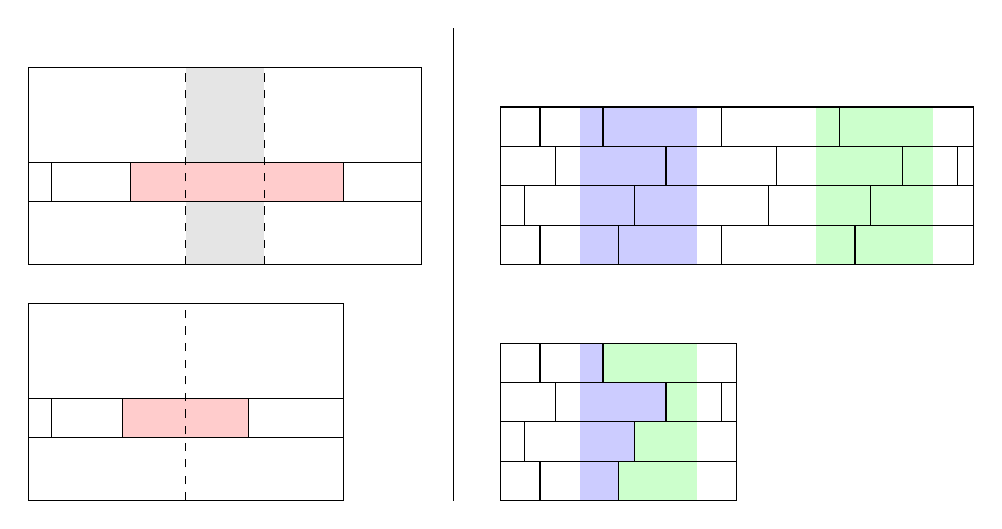
\begin{tikzpicture}
		\draw[white,fill=gray!20] (2,0) rectangle (3,0.8);
		\draw[white,fill=gray!20] (2,1.3) rectangle (3,2.5);
		
		\draw (0,0) rectangle (5,2.5);
		
		\draw (0,0.8) rectangle (5,1.3);
		
		\draw (0,0.8) rectangle (0.3,1.3);
		\draw (0,0.8) rectangle (1.3,1.3);
		\draw[fill=red!20] (1.3,0.8) rectangle (4,1.3);
		
		\draw[dashed] (2,0) -- (2,2.5);
		\draw[dashed] (3,0) -- (3,2.5);
		
		
		
		\draw (0,-3) rectangle (4,-0.5);
		
		\draw (0,-2.2) rectangle (4,-1.7);
		
		\draw (0,-2.2) rectangle (0.3,-1.7);
		\draw (0.3,-2.2) rectangle (1.3,-1.7);
		\draw[fill=red!20] (1.2,-2.2) rectangle (2.8,-1.7);
		
		\draw[dashed] (2,-3) -- (2,-0.5);
		
		\draw (5.4,-3) -- (5.4,3);
		
		
		\draw[white,fill=blue!20] (7,0) rectangle (8.5,2);
		\draw[white,fill=green!20] (10,0) rectangle (11.5,2);
		
		\draw (6,0) rectangle (12,2);
		
		\draw (6,0) rectangle (12,0.5);
		\draw (6,0) rectangle (12,1);
		\draw (6,0) rectangle (12,1.5);
		
		\draw (6,0) rectangle (6.5,0.5);
		\draw (6,0) rectangle (7.5,0.5);
		\draw (6,0) rectangle (8.8,0.5);
		\draw (6,0) rectangle (10.5,0.5);
		
		\draw (6,0.5) rectangle (6.3,1);
		\draw (6,0.5) rectangle (7.7,1);
		\draw (6,0.5) rectangle (9.4,1);
		\draw (6,0.5) rectangle (10.7,1);
		
		\draw (6,1) rectangle (6.7,1.5);
		\draw (6,1) rectangle (8.1,1.5);
		\draw (6,1) rectangle (9.5,1.5);
		\draw (6,1) rectangle (11.1,1.5);
		\draw (6,1) rectangle (11.8,1.5);
		
		\draw (6,1.5) rectangle (6.5,2);
		\draw (6,1.5) rectangle (7.3,2);
		\draw (6,1.5) rectangle (8.8,2);
		\draw (6,1.5) rectangle (10.3,2);
		
		
		\draw[white, fill=blue!20] (7,-3) rectangle (7.5,-2.5);
		\draw[white,fill=blue!20] (7,-2.5) rectangle (7.7,-2);
		\draw[white,fill=blue!20] (7,-2) rectangle (8.1,-1.5);
		\draw[white,fill=blue!20] (7,-1.5) rectangle (7.3,-1);
		
		\draw[white,fill=green!20] (7.5,-3) rectangle (8.5,-2.5);
		\draw[white,fill=green!20] (7.7,-2.5) rectangle (8.5,-2);
		\draw[white,fill=green!20] (8.1,-2) rectangle (8.5,-1.5);
		\draw[white,fill=green!20] (7.3,-1.5) rectangle (8.5,-1);
		
		
		
		\draw (6,-3) rectangle (9,-2.5);
		\draw (6,-3) rectangle (9,-2);
		\draw (6,-3) rectangle (9,-1.5);
		\draw (6,-3) rectangle (9,-1);
		
		\draw (6,-3) rectangle (6.5,-2.5);
		\draw (6,-3) rectangle (7.5,-2.5);
		
		\draw (6,-2.5) rectangle (6.3,-2);
		\draw (6,-2.5) rectangle (7.7,-2);
		
		\draw (6,-2) rectangle (6.7,-1.5);
		\draw (6,-2) rectangle (8.1,-1.5);
		\draw (6,-2) rectangle (8.8,-1.5);
		
		\draw (6,-1.5) rectangle (6.5,-1);
		\draw (6,-1.5) rectangle (7.3,-1);
		
	\end{tikzpicture}


% \caption{Illustration of the proof of Lemma~\ref{lem:short-local-runs}. Lines correspond to registers, and vertical separations are times at which the value of that register changes. If one register $i$ keeps the same value for a long enough time (on the left), we apply the induction hypothesis to shorten the projection of the run on the other registers. As the value of $i$ does not change, the resulting run is still valid. If all registers change values often (on the right), then if the run is long enough we can find two identical sequences of transitions during which all values are renewed. We can then obtain a shorter run by glueing them together as in the picture.}
% \end{figure}

\subsection{Local bounds}

\begin{lemma}
	\label{lem:short-local-runs}
	There exists a function $\towerfun(n, \regnum)$ in $O(\intro*\repexp{n}{\regnum})$ such that, for every protocol $\prot$ with $r$ registers per process, for every "local run" $\localrun: (q, \localdata) \step{*} (q', \localdata')$ in $\prot$, there exists $\localrun': (q, \localdata) \step{*} (q', \localdata')$ such that $\length{\localrun'} \leq \towerfun(\size{\prot})(r)$ and:
	\begin{enumerate}
		\item \label{item:shorterrun_anyvalue} for all $\aval' \in \nats$, there exists $\aval \in \nats$ such that $\vinput{\aval'}{\localrun'}$ is a subword of $\vinput{\aval}{\localrun}$,
		\item \label{item:shorterrun_oldvalues} for all $\aval \in \nats$ appearing in some message in $\localrun$, $\vinput{\aval}{\localrun'}$ is a subword of $\vinput{\aval}{\localrun}$. 
		% \item by writing $V := \nats \setminus \set{\localdata_i(k) \mid k \in \nset{1}{\regnum}}$, for every $\aval' \in V$, there exists $\aval \in V$ such that $\vinput{\aval'}{\localrun'}$ is a subword of $\vinput{\aval}{\localrun}$.
	\end{enumerate}
		%  with an "input" $I$.
% 	Let $u_1, u_2, u_3$ be such that $u=u_1u_2u_3$.
% 	If $\size{u_2} > TOWER$, then there exists $u'_2$ with $|u_2'| \leq \towerfun(\prot)$ such that $u_1u'_2u_3$ is a local run of $\prot$ with smaller "input" than $u$. 
\end{lemma}

\ifproofs
\begin{proof}

% In the following proof, we consider for simplicity protocols with internal transitions, \emph{i.e.}, transitions with no labeled action that can be taken without condition. 
Given a "local run" $\localrun$, register $i$ is ""active"" in $\localrun$ if at least one $\quotemarks{\enregact}$ step on register $i$ is performed in $\localrun$. Also, let $n:=\size{\prot}$.

We prove the ""shortening property"": \\
Let a "local run" $\localrun: (q_i, \localdata_i) \step{*} (q_f, \localdata_f)$ with $k$ "active registers" such that $\length{\localrun} > \towerfun(n,k)$ and let $V \subseteq \nats$ finite that contains every message value appearing in $\localrun$. We claim that $\localrun$ can be shortened into a local run $\localrun': (q_i, \localdata_i) \step{*} (q_f, \localdata_f)$ with $k$ active registers such that $\length{\localrun'} < \length{\localrun}$ and:
 \begin{itemize}
\item for all $\aval' \in \nats$, there exists $\aval \in \nats$ such that $\vinput{\aval'}{\localrun'}$ is a subword of $\vinput{\aval}{\localrun}$,
		\item for all $\aval \in V$, $\vinput{\aval}{\localrun'}$ is a subword of $\vinput{\aval}{\localrun}$. 
 \end{itemize}

We proceed by induction on the number $k$ of "active registers" in the "local run". If $k=0$, register values do not change in $\localrun$. Therefore, if $\localrun$ goes through the same state twice, all steps in between may be removed and it suffices to take $\towerfun(\size{\prot}, 0) := |\prot| + 1 \geq |Q| +1$.  

Suppose that the property is true for any protocol with $\leq k$ "active registers", and consider a run $\localrun: (q_i,\localdata_i) \step{*} (q_f,\localdata_f)$ with $k+1$ "active registers" such that $\length{\localrun} > \towerfun(n)(k+1)$.

First, if there exists an infix "local run" $\localrun_i$ of $\localrun$ of length $\towerfun(n)(k)+1$ with only $k$ active registers, then it suffices to apply the induction hypothesis on $u_i$ and $V$.

Suppose now that there exists no such infix "local run".
Let $I \subseteq \nset{1}{r}$ the set of "active registers" in $\localrun$, $|I| = k+1$. Let $M:= \towerfun(n)(k){+}1$. 
In any sequence of $M$ "local steps" in a row in $\localrun$, 
there is a $\quotemarks{\enregact}$ transition on every register in $I$. Let $\towerfun(n)(k+1) := M (n^{2M}+1)$ and suppose that $\length{\localrun} > \towerfun(n)(k+1)$. Additionally, suppose that $\localrun$ no local configuration appears twice in $\localrun$ (otherwise $\localrun$ may easily be shortened). For every $i$, let $\atrans_i$ the $i$-th transition in $\localrun$.
 For every $i \in \nset{0}{n^{2M}}$, we write $s_i$ the sequence $\delta_{2  M \cdot i+1}, \delta_{2  M \cdot i+2}, \cdots, \delta_{2 M \cdot i+2M}$.
By Pigeonhole principle two of the sequences $s_i$ are equal (there are $|\transitions|^{2M}$ distinct such sequences and $|\transitions| \leq n$). 
There exist two infix "local runs" $\localrun_a: (q_1, \localdata_1) \step{*} (q_2, \localdata_2)$, $\localrun_b: (q_3, \localdata_3) \step{*} (q_4, \localdata_4)$ in $\localrun$ such that $(q_2,\localdata_2)$ appears strictly before $(q_3,\localdata_3)$ in $\localrun$ and $\localrun_a$ and $\localrun_b$ both have sequence of transitions $s$.

Although $\localrun_a$ and $\localrun_b$ have the same sequence of transitions, their schedules may differ because their "external messages" may have different values.
We build a schedule $\sigma$ such that $(q_1,\localdata_1) \step{\sigma} (q_4, \localdata_4)$ where the underlying sequence of transitions of $\sigma$ is $s$.

For every active register $i \in I$, let $e_i \in \nset{1}{2M}$ denote the index of the first $\quotemarks{\enregact}$ on register $i$ in $s$ and $f_i \in \nset{1}{2M}$ the index of the last $\quotemarks{\enregact}$ on register $i$ in $s$. By hypothesis, because $s$ is of length $2M$, it contains at least two $\quotemarks{\enregact}$ on register $i$, one in the fist half and one in the second half, hence $e_i \leq M < M +1 \leq f_i$. 

For every $j \in \nset{1}{2M}$, let $\delta_j$ denote the $j$-th transition of $s$. First, if  $\delta_j$ is a "broadcast" or a "local test", we define the $j$-th "local step" of $\sigma$ as $\intlabel{\delta_j}$. 
Suppose now that $\delta_j$ is a "reception" of the form $\rec{\amessage}{i}{\anact}$. The $j$-th "local step" of $\localrun_a$ (resp. $\localrun_b$) has underlying transition $\delta_j$ hence is an "external message" of the form $\extlabel{\delta_j}{\aval_a}$ for some $\aval_a \in V$ (resp. $\extlabel{\delta_j}{\aval_b}$ for some $\aval_b \in V$).
Because $V$ is finite, there exists a function $\phi: V \rightarrow \nats \setminus V$ injective.
We define the $j$-th "local step" of $\sigma$ to be $\extlabel{\delta_j}{\aval}$ where:
\begin{itemize} 
\item if $j < e_i$, $\aval = \aval_a$,
\item if $e_i \leq j < f_i$, $\aval = \phi(\aval_a)$,
\item if $f_i \leq j$, $\aval = \aval_b$.
\end{itemize}
We now claim that $(q_1,\localdata_1) \step{\sigma} (q_4,\localdata_4)$. 
First, for every active register $i$, the last $\quotemarks{\enregact}$ step on register $i$ has value $\localdata_4(i)$ in $\sigma$ (as we are in the case $f_i \leq j$). Hence if every "local step" is valid then the final "local configuration" is $(q_4, \localdata_4)$.
For every $l \in \nset{0}{2M}$, let $\sigma_l$ denote the prefix of $\sigma$ of length $l$.
We prove by induction on $l$ that $\sigma_l$ is valid from $(q_1, \localdata_1)$. It is trivially true for $l =0$. Assume that we have $(q_1, \localdata_1) \step{\sigma_l} (q, \localdata)$ and let $\locallabel$ such that $\sigma_l \cdot \locallabel = \sigma_{l+1}$. Let $\atrans$ the underlying transition of $\locallabel$.
First, $q$ is the initial state of $\atrans$ because $\locallabel$ is valid at step $l+1$ of $\localrun_a$ (and $\localrun_b$). Hence if $\atrans$ is a "broadcast" then $\locallabel$ is valid from $(q,\localdata)$.

For every $i \in I$, let $\localdata_a, \localdata_b$ the content of register $i$ after the $l$-th step in $\localrun_a$ and $\localrun_b$ respectively.

\noindent \textbf{$\locallabel$ is an "external message"} \\
If $\locallabel$ is an "external message" of the form $\extlabel{\atrans}{\aval}$, then $\atrans$ has action $\rec{\amessage}{i}{\anact}$. Let $\aval_a$, $\aval_b$ the value of the corresponding "external message" in $\localrun_a$ and $\localrun_b$ respectively. The only problematic cases are when $\anact = \quotemarks{\diseqtestact}$ or $\anact = \quotemarks{\eqtestact}$.

In this case, we prove that $\binrel{\aval}{\anact}{\localdata(i)}$ with $\anact \in \set{\quotemarks{\eqtestact}, \quotemarks{\diseqtestact}}$. First, because the corresponding step is valid in $\localrun_a$ and $\localrun_b$, we have $\binrel{\localdata_a(i)}{\anact}{\aval_a}$ and $\binrel{\localdata_b(i)}{\anact}{\aval_b}$. We distinguish cases depending on the value of $l+1$:
\begin{itemize}
\item $l+1<e_i$: $\localdata(i)= \localdata_a(i)$, $\aval = \aval_a$ and $\binrel{\localdata_a(i)}{\anact}{\aval_a}$. 
\item $e_i \leq l+1 < f_i$: We have $\aval = \phi(\aval_a)$. 
Moreover, because $e_i < l+1$, there is at least one $\quotemarks{\enregact}$ on register $i$ in $\sigma_l$. Consider the last such "transition" in $\sigma_l$; its index $j$ satisfies $e_i \leq j < f_i$ by definition of $e_i$, hence the value of the corresponding "external message" in $\localrun_a$ is $\localdata_a(i)$ and its value in $\sigma_{l}$ is $\phi(\localdata_a(i))$. One has $\binrel{\localdata_a(i)}{\anact}{\aval_a}$ therefore (by injectivity of $\phi$ for $\anact = \quotemarks{\diseqtestact}$)
 $\binrel{\phi(\localdata_a(i))}{\anact}{\phi(\aval_a)}$.
\item$f_i \leq l+1$: $\localdata(i)= \localdata_b(i)$ and $\aval = \aval_b$, and because the "internal step" is valid in $\localrun_b$ we have $\binrel{\localdata_b(i)}{\anact}{\aval_b}$. 
\end{itemize}

\noindent \textbf{$\locallabel$ is an "internal step"} \\
The only problematic case is when $\locallabel =: \loc{i}{i'}{\diseqtestact}$ with $i,i' \in \nset{1}{\regnum}$ (we have no equality tests thanks to Lemma~\ref{lem:simple-reduction}). We have to prove that $\localdata(i) \ne \localdata(i')$. 
Because the "local test" is satisfied in $\localrun_a$ and $\localrun_b$, we have $\localdata_a(i) \ne \localdata_a(i')$ and $\localdata_b(i) \ne \localdata_b(i')$.

If $i \notin I$ and $i' \notin I$ (none are "active registers") then  $\localdata(i) = \localdata_a(i) \ne \localdata_a(i') = \localdata(i')$.

If $i \in I$ and $i' \notin I$, then $\localdata(i') = \localdata_a(i') = \localdata_b(i')$ and:
\begin{itemize}
\item if $l+1<e_i$ then $\localdata(i) = \localdata_a(i) \ne \localdata_a(i')$,
\item if $e_i \leq l+1 < f_i$ then $\localdata(i) = \phi(\localdata_a(i)) \notin V$ and  $\localdata(i') \in V$ therefore $\localdata(i) \ne \localdata(i')$,
\item if $f_i \leq l+1$ then $\localdata(i) = \localdata_b(i) \ne \localdata_b(i')$.
\end{itemize}
We treat the case $i \notin I$ and $i' \in I$ symmetrically.

If $i \in I$ and $i' \in I$, recall that $e_i \leq M < f_{i'}$ and $e_{i'} \leq M < f_i$ thus $e_i < f_{i'}$ and $e_{i'}< f_i$. We again make a case disjunction on the value of $l+1$:
\begin{itemize}
\item $l+1<e_i$ and $l+1 <e_{i'}$: $\localdata(i)= \localdata_a(i)$, $\localdata(i)= \localdata_a(i)$ and $\localdata_a(i) \ne \localdata_a(i')$. 
\item $e_i \leq l+1 < f_i$, $l+1<e_{i'}$: $\localdata(i) = \phi(\localdata_a(i)) \notin V$, $\localdata(i') = \localdata_a(i') \in V$ therefore $\localdata(i') \ne \localdata(i)$.
\item $e_{i'} \leq l+1 < f_{i'}$, $l+1<e_{i}$: symmetric to the previous case.
\item $e_i \leq l+1 < f_i$, $e_{i'} \leq l+1 < f_{i'}$: $\localdata(i) = \phi(\localdata_a(i))$, $\localdata(i') = \phi(\localdata_a(i'))$; however $\localdata_a(i) \ne \localdata_a(i')$ and $\phi$ is injective hence $\localdata(i') \ne \localdata(i)$.
\item $e_i \leq l+1 < f_i$, $f_{i'} \leq l+1$: $\localdata(i') = \localdata_b(i') \in V$, $\localdata(i) = \phi(\localdata_a(i)) \notin V$ hence $\localdata(i) \ne \localdata(i')$.
\item $f_i \leq l+1$, $e_{i'} \leq l+1 < f_{i'}$: symmetric to the previous case.
\item $f_i \leq l+1$, $f_{i'} \leq l+1$: $\localdata(i)= \localdata_b(i)$, $\localdata(i)= \localdata_b(i)$ and $\localdata_b(i) \ne \localdata_b(i')$. 
\end{itemize}

This proves that $\locallabel$ is valid from $(q,\localdata)$ which concludes the induction. 
We have proven that $(q_1,\localdata_1) \step{\sigma} (q_4, \localdata_4)$; however $\sigma$ is of length $2M$ and there are at least $2M+1$ steps between $(q_1,\localdata_1)$ and $(q_4, \localdata_4)$ in $\localrun$. Therefore, replacing this part of $\localrun$ with $(q_1,\localdata_1) \step{\sigma} (q_4, \localdata_4)$ yields a "local run" $\localrun': (q_i, \localdata_i) \step{*} (q_f,\localdata_f)$ with strictly less steps that $\localrun$. 

It remains to prove the conditions on the "$v$-inputs" of $\localrun'$. If suffices to prove the condition for the part between $(q_1, \localdata_1)$ to $(q_4, \localdata_4)$,
 because the rest of $\localrun$ is left untouched. 

Let $(q_m, \localdata_m)$ the "local configuration" after $M$ steps of $\sigma$ from $(q_1, \localdata_1)$; write $\localrun_1$ the local run from $(q_1,\localdata_1)$ to $(q_m, \localdata_m)$ corresponding to the first $M$ steps of $\sigma$ in $\localrun'$, and $\localrun_2$ the "local run" from $(q_m, \localdata_m)$ to $(q_4, \localdata_4)$ corresponding to the last $M$ steps of $\sigma$ in $\localrun'$.  

Let $\aval \in V$. We claim that $\vinput{\aval}{\localrun_{1}}$ is a subword of $\vinput{\aval}{\localrun_a}$ and $\vinput{\aval}{\localrun_{2}}$ is a subword of $\vinput{\aval}{\localrun_b}$. Indeed, in the construction of $\sigma$, the "external message" steps in the first $M$ steps were those of $\localrun_a$ except that some values were replaced with fresh values in $\nats \setminus V$, and similarly with $\localrun_b$ and the last $M$ steps. Overall, this proves that $\vinput{\aval}{\localrun'}$ is a subword of $\vinput{\aval}{\localrun}$ for every $\aval \in V$ and values of $V$ satisfy conditions \ref{item:shorterrun_anyvalue} and \ref{item:shorterrun_oldvalues}. 

Let $\aval' \in \nats \setminus V$; $\aval$ does not appear in $\localrun$. Either $\aval'$ does not appear in $\sigma$ in which case the desired property is true, or there exists $\aval \in V$ such that $\aval' = \phi(\aval)$. But then $\vinput{\aval'}{\localrun_{1}}$ is a subword of $\vinput{\aval}{\localrun_a}$ and $\vinput{\aval'}{\localrun_{2}}$ is a subword of $\vinput{\aval}{\localrun_b}$. Indeed, in $\localrun_1$, the "external message" steps with value $\phi(\aval)$ correspond to "external message" steps in $\localrun_a$ with value $\aval$, and similarly for $\localrun_2$ and $\localrun_b$. This proves condition \ref{item:shorterrun_anyvalue} for every $\aval' \in \nats \setminus V$.
Overall, we have proven the existence of a "local run" $\localrun': (q_i,\localdata_i) \step{*} (q_f,\localdata_f)$ that satisfies conditions \ref{item:shorterrun_anyvalue} and \ref{item:shorterrun_oldvalues} and that is strictly shorter that $\localrun$, which proves the "shortening property".

We build a "local run" of length strictly less that $\towerfun(\size{\prot})(\regnum)$ as follows. We start with $\localrun^{(0)} := \localrun$ and $V^{(0)}$ the set of values of messages appearing in $\localrun^{(0)}$. For every $k$ such that $\length{\localrun^{(0)}} > \towerfun(\size{\prot})(\regnum)$, we apply the "shortening property" on $\localrun^{(k)}$ and $V^{(k)}$ to obtain $\localrun^{(k+1)}$ and define $V^{(k+1)}$ by $V^{(k)} \cup W$ where $W$ is the set of values of messages in $\localrun^{(k+1)}$, which is finite.
The construction stops when $\length{\localrun^{(k)}} \leq \towerfun(\size{\prot})(\regnum)$, which concludes the proof of Lemma~\ref{lem:short-local-runs}. 	


%Overall, we have proven the existence of a "local run" $\localrun': (q_i,\localdata_i) \step{*} (q_f,\localdata_f)$ that satisfies the properties on the "$v$-inputs" and that is strictly shorter that $\localrun$. This process may be iterated to obtain a "local run" of length strictly less that $\towerfun(\size{\prot})(\regnum)$; on further iterations, one must simply make sure that fresh values chosen by $\phi$ appear in no message of previous iterations, \emph{i.e.}, that $V$ only increases at each iteration.	

\end{proof}
\fi 

\begin{remark}
	The tower bound of Lemma~\ref{lem:short-local-runs} is tight, in the sense that some local runs may need to have length a tower of exponentials of linear height in the number of registers.
	It also holds for pushdown automata, and for all transition systems which have some kind of pumping lemma.
	\cortoin{To formalize}
\end{remark}


\begin{lemma}
	\label{lem:short-run-for-output}
	Let $\prot$ be a "protocol", $\localrun$ a local run of $\prot$. 
	Let $w_{in} \in (\messages\times \nats)^*$ be a subword of $\Output{\localrun}$.
	
	Then there is a run $\localrun'$ of $\prot$ such that $\size{\localrun'}\leq \size{w_{in}} (\towerfun(\size{\prot})(r) +1)$, $w_{in} \subword \Output{\localrun'}$ and  
	\begin{enumerate}
		\item for all $\aval' \in \nats$, there exists $\aval \in \nats$ such that $\vinput{\aval'}{\localrun'}$ is a subword of $\vinput{\aval}{\localrun}$,
		\item for all $\aval \in \nats$ appearing in some message in $\localrun$, $\vinput{\aval}{\localrun'}$ is a subword of $\vinput{\aval}{\localrun}$. 
	\end{enumerate}
\end{lemma}

\begin{proof}
	Let $(m_1, v_1) \cdots (m_k, v_k) = w_{in}$, as $w_{in} \subword \Output{\localrun}$ we can split $\localrun$ into $(q_0, \nu_0) \step{u_1} (q'_1, \nu'_1) \intstep{\delta_1} (q_1, \nu_1) \step{u_2} (q'_2, \nu'_2) \intstep{\delta_2} (q_2, \nu_2) \cdots \step{u_k}  (q'_k, \nu'_k) \intstep{\delta_k} (q_k, \nu_k) \step{u_{k+1}} (q'_{k+1}, \nu'_{k+1})$ where for all $j \in [1,k]$ $\delta_i$ applies a broadcast operation $\br{m_j}{i_j}$ with $\nu'_{j} (i_j) = v_j$.
	
	By Lemma~\ref{lem:short-local-runs}, for all $j \in [1,k]$ there exists a run $\Tilde{\localrun}_j$ of length $\length{\Tilde{\localrun}_j} \leq \towerfun(\size{\prot})(r)$ from $(q_{j-1}, \nu_{j-1})$ to $(q'_{j}, \nu'_{j})$ such that for all $v' \in \nats$, either $\vinput{v'}{\Tilde{\localrun}_j} \subword \vinput{v'}{\localrun_j}$ or $v'$ does not appear in $\localrun_j$ and there exists $v \in \nats$ such that $\vinput{v'}{\Tilde{\localrun}_j} \subword \vinput{v}{\localrun_j}$.
	
	For each $j$, we can apply an injective renaming to the values in $\Tilde{\localrun}_j$ so that all values appearing in the "local configurations" $(q_{j-1}, \nu_{j-1})$ and $(q'_{j}, \nu'_{j})$ stay the same and all others are mapped to fresh distinct values. We call the resulting run $\localrun'_j$.
	
	This way all values appearing in $\localrun'_j$ only appear there, besides those in $(q_{j-1}, \nu_{j-1})$ and $(q'_{j}, \nu'_{j})$. As the values in the start and end configurations are the same, $\localrun'_j$ is still a "local run" from $(q_{j-1}, \nu_{j-1})$ to $(q'_{j}, \nu'_{j})$. Further, for all $v' \in \nats$,
	\begin{itemize}
		\item either $v'$ appears in $(q_{j-1}, \nu_{j-1})$ or $(q'_{j}, \nu'_{j})$, hence in $\localrun_j$, and $\vinput{v'}{\localrun'_j} = \vinput{v'}{\Tilde{\localrun}_j} \subword \vinput{v'}{\localrun_j}$,
		
		\item or $v'$ does not appear in $(q_{j-1}, \nu_{j-1})$ or $(q'_{j}, \nu'_{j})$, hence by definition of $\localrun'_j$ it is a fresh value \corto{define fresh} and in particular it does not appear in $\localrun_j$. There exists a value $\Tilde{v}$ of $\Tilde{\localrun}$ such that $\vinput{v'}{\localrun'} = \vinput{\Tilde{v}}{\Tilde{\localrun}}$ and by definition of $\Tilde{\localrun}$ there exists $v$ such that $\vinput{\Tilde{v}}{\Tilde{\localrun}_j} \subword \vinput{v}{\localrun_j}$, thus $\vinput{v'}{\localrun'_j} \subword \vinput{v}{\localrun_j}$.
	\end{itemize}

	We now define $\localrun'$ as $(q_0, \nu_0) \step{u'_1} (q'_1, \nu'_1) \intstep{\delta_1} (q_1, \nu_1) \step{u'_2} (q'_2, \nu'_2) \intstep{\delta_2} (q_2, \nu_2) \cdots \step{u'_k}  (q'_k, \nu'_k) \intstep{\delta_k} (q_k, \nu_k)$. As the local steps $(q'_j, \nu'_j) \intstep{\delta_j} (q_j, \nu_j)$ are unchanged, we have $w_{in} \subword \Output{\localrun}$.
	The length of $\localrun'$ is $k + \sum_{j=1}^{k} \length{u'_j} \leq \size{w_{in}} (\towerfun(\size{\prot})(r) +1)$.
	
	Moreover, for all $v' \in \nats$, 
	\begin{itemize}
		\item either $v'$ appears in $\localrun$, then for all $j$ 
		\begin{itemize}
			\item either $v'$ appears in $(q_{j-1}, \nu_{j-1})$ or $(q'_{j}, \nu'_{j})$, in which case it appears in $\localrun_j$ hence $\vinput{v'}{\localrun'_j} \subword \vinput{v'}{\localrun_j}$,
			
			\item or $v'$ does not appear in $(q_{j-1}, \nu_{j-1})$ or $(q'_{j}, \nu'_{j})$, hence $\vinput{v'}{\localrun'_j} = \epsilon$ after the renaming.
		\end{itemize}
		As a consequence, for all $j$ we have $\vinput{v'}{\localrun'_j} \subword \vinput{v'}{\localrun_j}$, thus $\vinput{v'}{\localrun'} \subword \vinput{v'}{\localrun}$.
		
		\item or $v'$ does not appear in $\localrun$, thus by definition of $\localrun'_j$ it appears in at most one of the $\localrun'_j$ and if there is such a $j$ then there exists $v \in \nats$ such that $\vinput{v'}{\localrun'_j} \subword \vinput{v}{\localrun_j}$, hence $\vinput{v'}{\localrun'} \subword \vinput{v}{\localrun}$.
	\end{itemize}
	This concludes our proof.
\end{proof}

\begin{lemma}
	\label{lem:short-dec}
	Let $\decsymb = (w_0, m_1, \ldots, w_\ell)$ be a decomposition, and for all $i\in [0,\ell]$ let $\decsymb_i = (w_0, m_1, \ldots, w_i)$.
	Let $w'_0, \ldots, w'_\ell$ be such that $w'_i \in \langdecdown{\decsymb_i}$ for all $i$.
	
	Then there exists $\widehat{\decsymb} = (\widehat{w}_0, m_1, \ldots, \widehat{w}_\ell)$ such that, for all $i$, $\widehat{w}_i \subword w_i$ and $w'_i \in \langdecdown{\widehat{\decsymb}_i}$ (where $\widehat{\decsymb}_i = (\widehat{w}_0, m_1, \ldots, \widehat{w}_\ell)$), and $\sum_{i=0}^{\ell} \size{\widehat{w}_i} \leq \sum_{i=0}^{\ell} \size{w'_i}$. 
\end{lemma}

\begin{proof}
	For all $i$, as $w'_i \in \langdecdown{\decsymb_i}$, we can split $w'_i$ into $v_{i,0} \cdots v_{i,i}$ where, for all $j$, $\wordproj{v_{i,j}}{\messages\setminus\set{m_1, \ldots, m_{j}}}$ is a subword of $w_j$. \corto{define pi as word projection}
	
	For all $j \in [0, \ell]$, for all $i\geq j$, $\wordproj{v_{i,j}}{\messages\setminus\set{m_1, \ldots, m_{j}}}$ is a subword of $w_j$.
	Hence we can find a subword $\widehat{w}_j$ of $w_j$ of size at most $\sum_{i=0}^{j} \size{\wordproj{v_{i,j}}{\messages\setminus\set{m_1, \ldots, m_{j}}}}$ such that $\wordproj{v_{i,j}}{\messages\setminus\set{m_1, \ldots, m_{j}}}$ is a subword of $\widehat{w}_j$ for all $i$, by considering for each $i$ a set of positions in $w_j$ that forms $\wordproj{v_{i,j}}{\messages\setminus\set{m_1, \ldots, m_{j}}}$, and then setting $\widehat{w}_j$ as the word formed by the union of those sets of positions.

	We then define $\widehat{\decsymb} = (\widehat{w}_0, m_1, \ldots, \widehat{w}_\ell)$ and for all $i$ $\widehat{\decsymb}_i = (\widehat{w}_0, m_1, \ldots, \widehat{w}_\ell)$.
	
	We obtain that for all $i$, $w'_i = v_{i,0} \cdots v_{i,i}$ with, for all $j \in [0,i]$, $\wordproj{v_{i,j}}{\messages\setminus\set{m_1, \ldots, m_j}} \subword \widehat{w}_j$. Hence we have $w'_i \in \langdecdown{\decsymb_i}$.
	
	Furthermore we have $\sum_{i=0}^{\ell} \size{\widehat{w}_i} \leq \sum_{i=0}^{\ell} \sum_{j=0}^i \size{v_{i,j}} = \sum_{i=0}^{\ell} \size{w'_i}$.
\end{proof}


\begin{lemma}
	\label{lem:bound-successor-height}
	Let $\prot$ be a "protocol", let $\node$ be a node of a "tree unfolding" $\tree$ of minimal size labelled by $\prot$ satisfying a "boss specification" $w$.
	Let $\node_1, \ldots, \node_k$ be its "follower" children. If $\node$ is not the root of $\tree$ then let $\mu'$ be its father.
	We have the following properties:
	
	\begin{enumerate}
		\item $k \leq \size{\messages}r$ \corto{correct in following proofs}
		
		\item The root of $\tree$ is a "boss node".
				
		\item  If $\node$ is a "boss node" then 
		\begin{itemize}
			\item If $\node$ is the root of $\tree$ then $\bosslabel{\node} = w$
			
			\item If $\node$ is not the root then $\size{\bosslabel{\node}} \leq \size{\localrunlabel{\node'}}$
			
			\item In both cases $\size{\localrunlabel{\node}} \leq (\towerfun(\size{\prot})(r) + 1)\Big[ \size{\bosslabel{\node}} + \sum_{i=1}^k \size{\followlabelword{\node_i}} \Big]$
		\end{itemize}
	
		\item If $\node$ is a "follower node" then 
		\begin{itemize}			
			\item $\size{\followlabelword{\node}} \leq \size{\localrunlabel{\node}}$
			
			\item $\size{\localrunlabel{\node}} \leq (\towerfun(\size{\prot})(r) +1)\Big[ 1 + \sum_{i=1}^k \size{\followlabelword{\node_i}} \Big]$
			
		\end{itemize}
	\end{enumerate}
\end{lemma}

\ifproofs
\begin{proof}
	Let $\node$ be a node of $\tree$. \corto{properly define trees and nodes}
	Let $V$ be the set of "initial values" being broadcast or received in $\localrunlabel{\node}$. We have $\size{V}\leq r$ as there is at most one such value for each register.  
	
	For each $v \in V$, if $v \neq \valuelabel{\node}$ (resp. if $v = \valuelabel{\node}$), let $\decsymb_v = (w_{v,0}, m_{v,1}, \ldots, w_{v,\ell_v})$ be a "decomposition" and $\node_{v,1}, \ldots, \node_{v, \ell_v}$ "follower" children of $\node$ such that condition \ref{unfoldingC3.1} (resp. \ref{unfoldingC1}) is respected.
	
	We can delete all other "follower" children of $\node$ and still have a "tree unfolding" satisfying $w$ as the $\node_{v,i}$ suffice to satisfy conditions \ref{unfoldingC1} and \ref{unfoldingC3.1} and the other conditions do not depend on "follower" children.
	As we assumed $\tree$ to be of minimal size, $\node$ does not have "follower" children besides the $\node_{v,i}$. As $\size{V} \leq r$ and $\ell_v \leq \size{\messages}$ for all $v$ (by definition of a "decomposition", as the $(m_{v,i})_{1\leq i \leq \ell_v}$ are all distinct), $\node$ has at most $\size{\messages}r$ "follower" children, proving property 1.
	
	Property 2 follows immediately from the fact that $\tree$ satisfies a "boss specification" $w$, which by definition implies that its root is a "boss node".
	
	Let $\node$ be a "boss node". If $\node$ is the root, then as $\tree$ satisfies $w$ we have $w \subword \bosslabel{\node}$. If $w \neq \bosslabel{\node}$, we can replace $\bosslabel{\node}$ with $w$: As $w \subword \bosslabel{\node}$, for all "decomposition" $\decsymb$, if $\bosslabel{\node} \in \langdecdown{\decsymb}$ then $w \in \langdecdown{\decsymb}$, hence condition~\ref{unfoldingC1} is still satisfied, and the other conditions of a "tree unfolding" are unaffected by this change.
	Furthermore the resulting "tree unfolding" still satisfies $w$. This contradicts the minimality of $\tree$, hence we have $\bosslabel{\node} = w$.
	
	If $\node$ is not the root, then let $\node'$ be its father. 
	Let $V'$ be the set of non-initial values $v'$ of $\node'$ such that $\vinput{v'}{\localrunlabel{\node'}} \subword \bosslabel{\node}$.
	
	We can construct a subword $\bossspec'$ of $\bosslabel{\node}$ of length at most $\sum_{v' \in V'} \size{\vinput{v'}{\localrunlabel{\node'}}}$ such that all $\vinput{v'}{\localrunlabel{\node'}}$ are subwords of $\bossspec'$. It suffices to select for each $v'$ a set of positions in $\bosslabel{\node}$ forming $\vinput{v'}{\localrunlabel{\node'}}$, and then taking the word formed by the union of those sets of positions.
	Observe that we necessarily have $\sum_{v' \in V'} \size{\vinput{v'}{\localrunlabel{\node'}}} \leq \size{\localrunlabel{\node'}}$, thus $\size{\bossspec'} \leq \size{\localrunlabel{\node'}}$.
	
	Like in the previous case, as $\bossspec'$ is a subword of $\bosslabel{\node}$, for all "decomposition" $\decsymb$, if $\bosslabel{\node} \in \langdecdown{\decsymb}$ then $\bossspec' \in \langdecdown{\decsymb}$. As a result, condition~\ref{unfoldingC1} is still satisfied after switching the label $\bosslabel{\node}$ to $\bossspec'$. Furthermore, by definition of $V'$ and $\bossspec'$, for all non-initial value $v'$ in $\localrunlabel{\node'}$, if $\vinput{v'}{\localrunlabel{\node'}} \subword \bosslabel{\node}$ then  $\vinput{v'}{\localrunlabel{\node'}} \subword \bossspec'$, hence condition~\ref{unfoldingC3.2} is still satisfied as well. Other conditions are unaffected by this change.
	
	Hence if $\size{\bosslabel{\node}} > \size{\localrunlabel{\node'}}$ we can obtain a "tree unfolding" smaller than $\tree$ and satisfying $w$, contradicting the minimality of $\tree$. As a result, $\size{\bosslabel{\node}} \leq \size{\localrunlabel{\node'}}$.
	
	We have shown the first two points of property 3. For the third one, we isolate the broadcasts of $\localrunlabel{\node}$ that are necessary to satisfy the "tree unfolding conditions" and then bound the length of $\localrunlabel{\node}$ using Lemma~\ref{lem:short-run-for-output}.
	
	Let $v$ be an initial value of $\localrunlabel{\node}$. If $v = \valuelabel{\node}$ then by condition~\ref{unfoldingC1} there exists a "decomposition" $\decsymb_v = (w_{v,0}, m_{v,1}, \ldots, w_{v,\ell_v})$ and "follower" children $\node_1, \ldots, \node_{\ell_v}$ such that
	\begin{itemize}
		\item 
	\end{itemize}
	
	 $\voutput{v}{}$
	 for all $i$ $\followlabelword{\node_i} \in \langdecdown{\decsymb_{v,i}}$, with $\decsymb_{v,i}= (w_{v,0}, m_{v,1}, \ldots, w_{v,i-1})$, and $\followlabelmessage{\node_i} = m_i$. 
	
	By Lemma~\ref{lem:short-dec}, we can assume that $\sum_{i=0}^{\ell_v} \size{w_{v,i}} \leq \sum_{i=0}^{\ell_v} \followlabelword{\node_i}$ 
	\cortoin{TO FINISH}
\end{proof}
\fi

\subsection{Tree bounds}

\begin{definition}
	We define the ""altitude"" of a node $\node$, written $\altitude{\node}$, in a "tree unfolding" recursively as follows:
	\begin{itemize}
		\item The altitude of the root is $0$
		
		\item The altitude of a "boss node" is the altitude of its father minus one
		
		\item The altitude of a "follower node" is the altitude of its father plus one.
	\end{itemize}
\end{definition}

\begin{lemma}
	\label{lem:bound-length-at-height-h}
	Let $\prot$ be a protocol, let $\node$ be a node of a "tree unfolding" of minimal size labelled by $\prot$ satisfying a "boss specification" $w$.
	Let $\altmax$ be the maximal "altitude" in $\tau$, let $N = \size{w} + \size{\prot} +1$ and let $f_0 : \nats \to \nats$ be the function mapping each $n \in \nats$ to $f_0(n)=(N^2 (\towerfun(N)(N) + 1))^{n+1}$ 
	
	\begin{itemize}
		\item If $\node$ is a "boss node" then $\size{\bosslabel{\node}} \leq f_0(\altmax - \altitude{\node}-1)$ and $\size{\localrunlabel{\node}} \leq f_0(\altmax - \altitude{\node})$.
		
		\item If $\node$ is a "follower node" then $\size{\localrunlabel{\node}} \leq \size{\followlabelword{\node}} \leq  f_0(\altmax - \altitude{\node})$.
	\end{itemize} 
	
	
	
\end{lemma}

\ifproofs
\begin{proof}
	We prove this by strong induction on $\altmax-\altitude{\node}$.
	
	Let $\node$ be a node, suppose that the inequalities hold for all nodes of greater "altitude". 
	Let $\node_1, \ldots, \node_k$ be its "follower" children. If $\node$ is not the root of $\tree$ then let $\mu'$ be its father.
	
	If it is a "boss node" then by Lemma~\ref{lem:bound-successor-height} if it is the root we have $\size{\bosslabel{\node}} = \size{w} \leq N$, and if not we have $\size{\bosslabel{\node}} \leq \size{\localrunlabel{\node'}} \leq f_0(\altmax - \altitude{\node} -1)$ by induction hypothesis. In both cases we have $\size{\bosslabel{\node}} \leq f_0(\altmax - \altitude{\node} -1)$.	
	In all cases we obtain $\size{\localrunlabel{\node}} \leq (\towerfun(\size{\prot})(r)+1) \Big[f_0(\altmax-\altitude{\node} -1) + \sum_{i=1}^k \size{\followlabelword{\node_i}}\Big]$
	
	By Lemma~\ref{lem:bound-successor-height} we have $k \leq \size{\messages}(r+1)$.
	Moreover, by induction hypothesis for all $i$ we have 
	$\size{\followlabelword{\node_i}} \leq f_0(\altmax-\altitude{\node} -1)$. As a result,
	
	$\size{\localrunlabel{\node}} \leq (\towerfun(\size{\prot})(r)+1) f_0(\altmax-\altitude{\node} -1)(\size{\messages} (r+1) +1) \leq N^2(\towerfun(N)(N) +1) f_0(\altmax - \altitude{\node} -1) \leq f_0(\altmax - \altitude{\node})$.
	
	If $\node$ is a "follower node" then by Lemma~\ref{lem:bound-successor-height} we have 
	$\size{\followlabelword{\node}} \leq \size{\localrunlabel{\node}} \leq \towerfun(\size{\prot})(r) +1 \leq f_0(\altmax - \altitude{\node})$.
\end{proof}
\fi

\begin{lemma}
	\label{lem:bound-max-height}
	There exists a function $f_1$ of the class $\Falpha{\omega^{\size{\messages}}}$ such that for all "protocol" $\prot$, for all "tree unfolding" $\tree$ of minimal size labelled by $\prot$ satisfying a "boss specification" $w$, the maximal altitude of a node of $\tree$ is bounded by $f_1(\size{\prot} + \size{w}+1)$.
\end{lemma}

\ifproofs
\begin{proof}
	Let $\tree$ be a "tree unfolding" of minimal size labelled by $\prot$ satisfying a "boss specification" $w$. Let $\altmax$ be the maximal altitude of a node in $\tree$. Let $\node_0, \ldots, \node_m$ be nodes of $\tree$ such that $\node_0$ is its root, $\altitude{\node_m} = \altmax$, and for all $i\in [1, m]$, $\node_i$ is a child of $\node_{i-1}$.
	For all $a \in [1, \altmax]$, let $j_a$ be the minimal index such that $\altitude{\node_{j_a}} = a$. This index exists as $\altitude{\node_0} = 0$, $\altitude{\node_m} = \altmax$ and for all $i$, $\altitude{\node_{i}} \leq \altitude{\node_{i-1}}+1$.
	Furthermore as $j_a$ is the minimal such index, we cannot have $\altitude{\node_j} \geq a$ for any $j < j_a$ as otherwise there would be a $j'$ such that $j' \leq j < j_a$ with $\altitude{\node_{j'}} = a$.
	
	As a consequence, we have $j_1 < j_2 < \ldots < j_{\altmax}$. Moreover, $\node_{j_a}$ is necessarily a "follower node" as otherwise we would have $\altitude{\node_{j_a-1}} = a+1 \geq a$.
	
	Let $\#$ be a fresh letter, and let $N = \size{w} + \size{\prot}+1$. For all $i \in [1, \altmax]$ let $\node'_i = \node_{j_{\altmax - i+1}}$ and $w_i = \followlabelword{\node'_{i}} \# \followlabelmessage{\node'_{i}} \in (\messages \cup \set{\#})^*$.
	
	We claim that we cannot have $w_{i_1}\subword w_{i_2}$ for any  $i_1< i_2$.
	Suppose by contradiction that there exist such $i_1$ and $i_2$ with $i_1 < i_2$. Then we would have $\followlabelword{\node'_{i_1}} \subword \followlabelword{\node'_{i_2}}$ and $\followlabelmessage{\node'_{i_1}} = \followlabelword{\node'_{i_2}}$.
	Therefore, as $\node_{i_1}$ is a descendant of $\node_{i_2}$, by Lemma~\ref{lem:increasing-followers} there would exist a "tree unfolding" of smaller size than $\tree$ satisfying $w$, contradicting the minimality of $\tree$.
	
	As a result, the sequence $(w_i){1\leq i \leq \altmax}$ is a "bad sequence" for the "subword normed well-quasi order" over the alphabet $\messages\cup\set{\#}$.
	Furthermore, by Lemma~\ref{lem:bound-length-at-height-h}, for all $i$, as $\altitude{\node'_{i}} = \altmax-i+1$, we have $\size{\followlabelword{\node_{j_a}}} \leq f_0(\altmax-i+1) = (N^2(\towerfun(N)(N)+1))^{i}$.
	
	Let $g$ be the function such that $g(n) = (n^2(\towerfun(n)(n)+1))n+2$. Clearly for all $i\geq 1$ we have $g^{(i)}(N) \geq (N^2(\towerfun(N)(N)+1))^{i} \geq N$.
	As a consequence, for all $a$, $\size{w_i} \leq (N^2(\towerfun(N)(N)+1))^{i} + 2 \leq (N^2(\towerfun(N)(N)+1)) g^{(i-1)}(N) + 2 \leq g^{(i)}(N)$
	
	By Theorem 5.3 in \cite{SchmitzS2011upperHigman}, there exists a function $f_1 \in \Falpha{\omega^{\size{\messages}}}$ such that all  "bad sequences" of words "controlled by" $(g,N)$ have at most $f_1(N)$ elements.
	
	Hence the sequence $(w_i){1\leq i \leq \altmax}$ cannot have more than $f_1(N) = f_1(\size{\prot} + \size{w} + 1)$ elements, thus $\altmax \leq f_1(\size{\prot} + \size{w} + 1)$.
\end{proof}
\fi


\begin{lemma}
	\label{lem:bound-min-height}
	There exists a function $f_2$ of the class $\Falpha{\omega^{\size{\messages}}}$ such that for all "protocol" $\prot$, for all "tree unfolding" $\tree$ of minimal size labelled by $\prot$ satisfying a "boss specification" $w$, the absolute value of the minimal "altitude" of a node of $\tree$ is bounded by $f_2(\size{\prot} + \size{w}+1)$.
\end{lemma}

\ifproofs
\begin{proof}
	We proceed similarly as in the proof of Lemma~\ref{lem:bound-max-height}. 
	
	Let $\tree$ be a "tree unfolding" of minimal size labelled by $\prot$ satisfying a "boss specification" $w$. Let $\altmin$ be the minimal altitude of a node in $\tree$. Let $\node_0, \ldots, \node_m$ be nodes of $\tree$ such that $\node_0$ is its root, $\altitude{\node_m} = \altmin$, and for all $i\in [1, m]$, $\node_i$ is a child of $\node_{i-1}$.
	For all $a \in [\altmin, 0]$, let $j_a$ be the minimal index such that $\altitude{\node_{j_a}} = a$. This index exists as $\altitude{\node_0} = 0$, $\altitude{\node_m} = \altmin$ and for all $i$, $\altitude{\node_{i}} \geq \altitude{\node_{i-1}}-1$.
	Furthermore as $j_a$ is the minimal such index, we cannot have $\altitude{\node_j} \leq a$ for any $j < j_a$ as otherwise there would be a $j'$ such that $j' \leq j < j_a$ with $\altitude{\node_{j'}} = a$.
	
	As a consequence, we have $j_0 < j_1 < j_2 < \ldots < j_{\altmin}$. Moreover, $\node_{j_a}$ is necessarily a "boss node" for all $a<0$ as otherwise we would have $\altitude{\node_{j_a-1}} = a-1 \leq a$, and $\node_{j_0}$ is the root and therefore also a "boss node" as $\tau$ satisfies $w$.
	
	Let $N = \size{w} + \size{\prot}+1$. For all $i \in [0, -\altmin]$ let $\node'_i = \node_{j_{-i}}$ and $w_i = \bosslabel{\node'_{i}} \in \messages^*$.
	
	We claim that we cannot have $w_{i_1}\subword w_{i_2}$ for any  $i_1< i_2$.
	Suppose by contradiction that there exist such $i_1$ and $i_2$ with $i_1 < i_2$. Then we would have $\bosslabel{\node'_{i_1}} \subword \bosslabel{\node'_{i_2}}$, hence, as $\node_{i_2}$ is a descendant of $\node_{i_1}$, by Lemma~\ref{lem:increasing-bosses} there would exist a "tree unfolding" of smaller size than $\tree$ satisfying $w$, contradicting the minimality of $\tree$.
	
	As a result, the sequence $(w_i){1\leq i \leq \altmax}$ is a "bad sequence" for the "subword normed well-quasi order" over the alphabet $\messages\cup\set{\#}$.
	By Lemma~\ref{lem:bound-length-at-height-h}, for all $\node'_i$ we have $\size{\bosslabel{\node'_i}} \leq f_0(\altmax - \altitude{\node'_i}) = f_0(\altmax +i)$.
	By Lemma~\ref{lem:bound-max-height}, we have $\altmax \leq f_1(N)$ and thus $\size{\bosslabel{\node'_i}} \leq  f_0(f_1(N) +i)$
	
	Let $g$ be the function such that $g(n) = (n^2(\towerfun(n)(n)+1))n+2$. 
	Let $M = f_0(f_1(N))$. Clearly for all $i\geq 0$ we have $g^{(i)}(M) \geq (N^2(\towerfun(N)(N)+1))^{f_1(N) + i}$.
	
	We have $\size{w_0} \leq M = g^{(0)}(N)$ and for all $i>0$, $\size{w_i} \leq (N^2(\towerfun(N)(N)+1))^{f_1(N) + i} + 2 \leq (N^2(\towerfun(N)(N)+1)) g^{(i-1)}(M) + 2 \leq g^{(i)}(M)$
	
	By definition of the function $f_1 \in \Falpha{\omega^{\size{\messages}}}$, all "bad sequences" of words "controlled by" $(g,N)$ have at most $f_1(N)$ elements.
	
	Hence the sequence $(w_i){1\leq i \leq \altmax}$ cannot have more than $f_1(M)$ elements, thus $\altmin \leq f_1(M) = f_1(f_0(f_1(N)))$.
	We define $f_2$ as $f_1 \circ f_0 \circ f_1$. It is a function of $\Falpha{\omega^{\size{\messages}}}$ as $f_0$ and $f_1$ are and $\Falpha{\omega^{\size{\messages}}}$ is closed by composition.
\end{proof}
\fi


\begin{corollary}
	\label{cor:bound-node-size}
	There exists a function $f_3$ of the class $\Falpha{\omega^{\size{\messages}}}$ such that for all "protocol" $\prot$, for all "tree unfolding" $\tree$ of minimal size labelled by $\prot$ satisfying a "boss specification" $w$, for all node $\node$ of $\tree$,
	
		\begin{itemize}
		\item $\size{\localrunlabel{\node}} \leq f_3(\size{\prot}+ \size{w})$
			
		\item If $\node$ is a "boss node" then $\size{\bosslabel{\node}} \leq f_3(\size{\prot}+ \size{w})$.
		
		\item If $\node$ is a "follower node" then $\size{\followlabelword{\node}} \leq f_3(\size{\prot}+ \size{w})$.
	\end{itemize} 
\end{corollary}

\ifproofs
\begin{proof}
	Consequence of Lemmas~\ref{lem:bound-length-at-height-h}, \ref{lem:bound-max-height} and \ref{lem:bound-min-height} as $\Falpha{\omega^{\size{\messages}}}$ is closed by composition.
\end{proof}
\fi


\begin{proposition}
	\label{prop:bound-tree-size}
	There exists a function $f_4$ of the class $\Falpha{\omega^{\size{\messages}}}$ such that for all "protocol" $\prot$, for all "tree unfolding" $\tree$ of minimal size labelled by $\prot$ satisfying a "boss specification" $w$, the size of $\tree$ is bounded by $f_4(\size{\prot} + \size{w}+1)$.
\end{proposition}

\ifproofs
\begin{proof}
	Let $\tree$ be a "tree unfolding" of minimal size labelled by $\prot$ satisfying a "boss specification" $w$. Let $N = \size{\prot} + \size{w}+1$.

	We first bound the height of $\tree$, then its arity (the maximal number of children of a node), which allows us to obtain a bound on the number of nodes.
	
	By Corollary~\ref{cor:bound-node-size}, for all "boss node" $\node$ in $\tree$ we have $\size{\bosslabel{\node}} \leq f_3(N)$.
	If a branch contains more than $\sum_{i=0}^{f_3(N)}\size{\messages}^{i}$ "follower nodes", then there are two nodes in it with the same "boss" label, hence $\tree$ can be reduced and still satisfy $w$, contradicting the minimality of $\tree$.
	
	Similarly, by Corollary~\ref{cor:bound-node-size}, for all "follower node" $\node$ in $\tree$ we have $\size{\followlabelword{\node}} \leq f_3(N)$.
	If a branch contains more than $\size{\messages}\sum_{i=0}^{f_3(N)}\size{\messages}^{i}$ "follower nodes", then there are two nodes in it with the same "follower" label, hence $\tree$ can be reduced and still satisfy $w$, contradicting the minimality of $\tree$.
	
	As a result, each branch of $\tree$ contains at most $1+ (\size{\messages}+1) \sum_{i=0}^{f_3(N)}\size{\messages}^{i}$ nodes. We simplify this expression: let $H = (f_3(N)+2)(N+1)^{f_3(N)+1}$, each branch of $\tree$ has at most $H$ nodes.
	
	Furthermore, by Lemma~\ref{lem:bound-successor-height}, each node has at most $\size{\messages}(r+1)$ "follower" children. We now bound its number of "boss" children.
	
	Let $\node$ be a node of $\tree$, let $V$ be the set of non-initial values appearing in $\localrunlabel{\node}$ apart from $\valuelabel{\node}$.
	By condition~\ref{unfoldingC3.2}, for each $v' \in V$, $\node$ has a "boss" child $\node_{v'}$ such that $\vinput{v'}{\localrunlabel{\node}} \subword \bosslabel{\node_{v'}}$.
	
	We simply observe that $\size{V} \leq \size{\localrunlabel{\node}}$ as every non-initial value needs to be received at some point in $\localrunlabel{\node}$. We also note that all other "boss" children of $\node$ can be removed, and the resulting tree still satisfies $w$ and is still a "tree unfolding". By minimality of $\tree$, this means that $\mu$ has at most $\size{\localrunlabel{\node}}$ "boss" children, hence at most $f_3(N)$ by Corollary~\ref{cor:bound-node-size}.
	
	As a consequence, each node in $\tree$ has at most $f_3(N) + \size{\messages}(r+1)$ children.
	
	By combining the bounds on the size of branches and the arity of nodes, we obtain that $\tree$ has at most $\sum_{h=0}^{H} (f_3(N) + \size{\messages}(r+1))^h$ nodes. We again simplify this: $\sum_{h=0}^{H} (f_3(N) + \size{\messages}(r+1))^h \leq (H+1)(f_3(N) + N^2)^H$.
	
	Finally, we obtain a bound on the size of $\tau$ by taking the product of the bounds on the number of nodes and on the size of each node label: 
	
	\[ \size{\tree} \leq  (H+1)(f_3(N) + N^2)^H (2f_3(N) +1)\]
	
	Let $f_4$ be such that $f_4(n) = ((f_3(n)+2)(n+1)^{f_3(n)+1} +1) (f_3(n) + n^2)^{(f_3(n)+2)(n+1)^{f_3(n)+1}}(2f_3(n) +1)$ for all $n$. It is the composition of $f_3$ with an elementary function, hence as $f_3 \in \Falpha{\omega^{\messages}}$ and $\Falpha{\omega^{\messages}}$ is closed by composition, $f_4 \in \Falpha{\omega^{\messages}}$.
	
	Furthermore, we have shown that the size of a minimal "tree unfolding" satisfying a "boss specification" $w$ and labelled by a "protocol" $\prot$ is bounded by $f_4(\size{\prot} + \size{w} +1)$.
\end{proof}
\fi



\subsection{Decidability}
\begin{theorem}
	The BNRA coverability problem is decidable in time $\Falpha{\omega^\omega}$ and there is no $\alpha < \omega^\omega$ such that this problem can be solved in time $\Falpha{\alpha}$.
	The lower bound holds even with two registers and no local tests.
\end{theorem}

\ifproofs
\begin{proof}
	The lower bound is given by the reduction from "lossy channel systems" reachability in Proposition~\ref{prop:reduction-LCS} and by the fact that there is no algorithm in time $\Falpha{\alpha}$ for LCS reachability with $\alpha < \omega^\omega$.
	
	For the upper bound, let $\prot$ be a "protocol" with $r \geq 1$ registers over messages $\messages$ and $q$ one of its states. We add a new message $m$ to $\messages$ and a new transition $\br{m}{1}$ from $q$ to itself broadcasting $m$. 
	
	Clearly the new "protocol" $\prot'$ satisfies the "boss specification" $m$ if and only if $q$ is coverable in $\prot$.
	
	By Lemmas~\ref{lem:run-to-tree} and \ref{lem:tree-to-run}, there is a run of $\prot'$ satisfying $m$ if and only if there is a "tree unfolding" satisfying $m$.
	
	By Lemma~\ref{prop:bound-tree-size}, there is such a "tree unfolding" if and only if there is one of size at most $f_4(\size{\prot}+2)$, where $f_4$ is a function of the class $\Falpha{\omega^{\size{\messages}}}$.
	
	The last problem we have is that the size of a "tree unfolding" does not take into account the values used in it. This can be solved by noticing that the conditions in the definition of a "tree unfolding" and the condition to satisfy a "specification" still hold after applying an injective renaming to the values. 
	
	Suppose there exists $\tree$ a "tree unfolding" satisfying $m$, let $V$ be the set of values appearing in that tree. In a node $\node$ the values appearing are
	\begin{itemize}
		\item $\valuelabel{\node}$
		
		\item The initial values of $\localrunlabel{\node}$ (there are $r$ such values)
		
		\item The non-initial values (at most $\size{\localrunlabel{\node}}$ as they all need to be received)
	\end{itemize}

	Hence there are at most $\size{\localrunlabel{\node}} + r +1$ different values appearing in each node.
	In total there are thus at most $\sum_{\node \in \tree} \size{\localrunlabel{\node}} + r +1$ different values in $\tree$, which is less than $(r+2)\size{\tree}$.
	
	We can apply an injective renaming $V \to [1,(r+2)\size{\tree}]$ to the values to obtain another "tree unfolding" satisfying $m$ and whose values do not exceed $(r+2)\size{\tree}$.
	
	Hence there exists a "tree unfolding" satisfying $m$ if and only if there is one of size at most $f_4(\size{\prot}+2)$ in which values do not exceed $f_4(\size{\prot}+2)$. A description of such a tree requires a space that is polynomial in its size.
	
	As a result, we can bound the size of the description of such a "tree unfolding" by a function of $\Falpha{\omega^{\size{\messages}}}$.
	An algorithm for the coverability problem thus consists in enumerating all trees labelled by local runs of $\prot$ of size at most $f_4(\size{\prot}+2)$ with values not exceeding $f_4(\size{\prot}+2)$, and accepting if and only if one of them satisfies the conditions to be a "tree unfolding" satisfying $m$.
	
	This can all be done in exponential time in $f_4(\size{\prot}+2)$, thus this algorithm terminates in time $f_5(\size{\prot})$ where $f_5$ is a function of $\Falpha{\omega^{\size{\messages}}}$.
	
	The BNRA coverability problem is thus decidable in time $\Falpha{\omega^\omega}$.
\end{proof}
\fi
